\documentclass{article}
\usepackage{import}
\usepackage[utf8]{inputenc}
\usepackage{amsmath}
\usepackage{amssymb}
\usepackage{mathtools}
\usepackage{graphicx}
\usepackage{tabularx}
\usepackage{float}
\usepackage{subfig}
\usepackage{lscape} 
\usepackage{hyperref}
\usepackage{setspace}
\usepackage{booktabs}
\usepackage[authoryear]{natbib}
\usepackage{lmodern}
\usepackage[T1]{fontenc}
\usepackage[bottom]{footmisc}
\newcommand{\indep}{\perp \!\!\! \perp}
\usepackage[nolist]{acronym}
\newcommand\headercell[1]{%
   \smash[b]{\begin{tabular}[t]{@{}c@{}} #1 \end{tabular}}}
\usepackage[a4paper,top=3cm,bottom=2cm,left=3cm,right=3cm,marginparwidth=1.75cm]{geometry}
\usepackage{xcolor}%
\definecolor{webbrown}{rgb}{.6,0,0}
\usepackage{hyperref}%
\hypersetup{%
  breaklinks = true,%
  colorlinks = true,%
  anchorcolor = webbrown,%
  citecolor = webbrown,%
  filecolor = webbrown,%
  linkcolor = webbrown,%
  menucolor = webbrown,%
  urlcolor= webbrown,%
  citebordercolor= 1 0 0,%
  menubordercolor=1 0 0,%
  urlbordercolor=1 0 0,%
  runbordercolor=1 0 0,}
\usepackage{cleveref}

\usepackage{setspace}
\usepackage{enumitem}
\setstretch{1.5} %% set line spacing

\begin{acronym}
  \acro{CI}{confidence interval}
  \acro{RCT}{randomized controlled trial}
  \acro{IV}{instrumental variable}
  \acro{LATE}{local average treatment effect}
  \acro{ATE}{average treatment effect}
  \acro{OLS}{ordinary least squares}
  \acro{RD}{regression discontinuity}
  \acro{MTE}{marginal treatment effect}
  \acro{ATT}{average treatment effect on the treated}
\end{acronym}

\graphicspath{ {../../output/figures/} }

% Wrap table notes
\usepackage{booktabs}
\newcommand{\tabnotes}[2]{\bottomrule \multicolumn{#1}{@{}p{0.70\linewidth}@{}}{\footnotesize #2 }\end{tabular}\end{table}}

\floatplacement{figure}{H}
\floatplacement{table}{H}

\usepackage[toc,page]{appendix}


\title{College Enrollment and Earnings:
\texorpdfstring{\\}{} Examining the Impact of Two Federal Drug Acts}
\author{Ray Huang\thanks{Contact:
    \href{mailto:ray_huang@brown.edu}{ray\_huang@brown.edu}.
     I thank Peter Hull at Brown University for serving as my advisor and for providing me with fantastic feedback and guidance. I would also like to thank Alison Lodermeier and Francesco Ferlenga for their generous comments and support. A replication archive with instructions is available at https://github.com/rayhuang11/EconSeniorThesisRH.}
     \\Brown University, Honors Thesis}

\date{\today}

\begin{document}

\maketitle

\begin{abstract}
\noindent I examine the impact of two federal drug acts on college enrollments and earnings among black males by using a variety of counterfactual groups. The Anti-Drug Act of 1986 transformed the formerly rehabilitation-focused justice system into a punitive one, imposed sentencing minimums and disparities. The Fair Sentencing Act of 2010 undid many of these policies. I construct estimates of the impact of these two acts on black males aged 18-24 using three unique counterfactual groups: 1) white males, 2) black females, and 3) black men aged 28-34. I also leverage the variation between high and low drug arrest states. I find that

\end{abstract}

\clearpage

\section{Introduction}

Anti-Drug Act of 1986:
\begin{itemize}[itemsep=0.05mm, parsep=0pt]
  \item Created minimum sentencing laws re possession of many drugs. 
  \item Crack/powdered cocaine was particularly relevant (significantly harder rules on crack, which was cheaper and used by minorities much more, 100-1 ratio)
  \item The law led to an increase in the average time imprisoned for drug crimes from 22 months to 33 months (Shewan)
\end{itemize}


Fair Sentencing Act of 2010:
\begin{itemize}[itemsep=0.05mm, parsep=0pt]
  \item Reduced the disparity between the amount of crack cocaine and powder cocaine needed to trigger certain federal criminal penalties from a 100:1 weight ratio to an 18:1 weight ratio 
  \item Elimated minimum sentencing for crack cocaine 
  \item Congressional Budget Office has estimated that implementing the Fair Sentencing Act of 2010 will reduce the prison population by 1,550 person-years over the period from 2011–2015, creating a monetary savings of \$42 million during that period 
\end{itemize}

Existing literature:
\begin{itemize}[itemsep=0.05mm, parsep=0pt]
  \item The Labor Market Consequences of Incarceration- Western, Kling, Weiman (2016)
  \item Juvenile Incarceration, Human Capital, and Future Crime: Evidence from Randomly Assigned Judges - Aizer, Doyle (2015)
  \item Evan Rose papers: The Impact of Incarceration on Employment and Earnings, etc
\end{itemize}



\section{Empirical Strategy}

I take three discrete approaches to my empirical strategy, establishing three unique counterfactual groups for identifying the impact of the Anti-Drug Abuse Act of 1986 and the Fair Sentencing Act of 2010 on college enrollment rates. 

My first empirical approach looks at changes in college enrollment rates in high drug arrest states relative to the low drug arrest states before and after the passage of both the 1986 and 2010 acts where high drug arrest states are defined as states above the 75th percentile two years before the passage of the federal law. I also utilize both the adult and juvenile arrest rates in two parallel analyses. I examine both the first-stage impact where the outcome is the change in drug-related arrest rates and the reduced-form impact where the outcome is college-enrollment. The first stage is evaluated using an event-study model that allows me to assess the evolution of relative outcomes while controlling for fixed differences across states and national trends over time. Using data at the state ($s$) by year ($t$) level, I estimate:

\begin{equation} \label{eq:state_level_es}
  y_{st} = \alpha_s + \gamma_t + X'_{st} \phi + \sum_{m=-G}^{M} \beta_m z_{s,t-m} + \epsilon_{st}
\end{equation}

where $\alpha_s$ and $\gamma_t$ are individual and time fixed effects, $X'_{st}$ is a vector of control variables, and $\epsilon_{st}$ represents a shock uncorrelated with the policy. The coefficients $\{\beta_m \}^{M}_{m=-G}$ summarize the magnitude of the dynamic effects and are summarized in an event-study plot.

In addition to the event study analyses, I also include traditional difference-in-differences estimates as a summary of the effect across all post-expansion years using the following regression specification at the individual ($i$) by year ($t$) level: 

\begin{equation} \label{eq:did}
  y_{it} = \alpha + \delta D_i + \gamma Post_t + \beta D_i Post_t + X'_{it}\phi + \epsilon_{it}
\end{equation}

where $D_{i}$ is an indicator for belonging to the treatment group (in this case, states with high drug arrests), $Post_t$ is a time indicator for belonging to the post-period, $D_i Post_t$ is the interaction term where $\beta$ is potentially the causal effect of the federal policy if the identifying assumptions are satisfied, and $X'_{it}$ is a vector of control variables.

My second and third empirical approaches mirror the approach taken in \cite {britton2022}. In my second empirical strategy, I look at changes in college enrollment rates in black males aged 18-24 at the time of the federal law passage relative to white males aged 18-24 at the time of the federal law passage.

My third approach is very similar to the second approach, where I look at the change in college enrollment rates in black males aged 18-24 at the time of the federal law passage relative to female blacks aged 18-24 at the time of the federal law passage.

Finally, I also include a triple difference-differences specification, where I compare

In all the regression specifications, I follow the recommendations outlined in \cite{duflo_did} and use robust standard errors clustered at the state level.

\textbf{Counterfactual groups}
\begin{itemize}[itemsep=0.05mm, parsep=0pt]
  \item Black males vs white males
  \begin{itemize}
    \item Identifying assumption: absent of the Anti-Drug Abuse Act of 1986, black and white male educational outcomes would have trended similarly.
  \end{itemize}
  \item Black males vs black females
  \item Black males aged 18-24 vs black males aged 28-34 at the time of the act
  \item High vs low drug use
\end{itemize}

\textbf{Empirical tools:}
\begin{itemize}[itemsep=0.05mm, parsep=0pt]
  \item DiD / DDD / Event study.
  \item \begin{itemize}
    \item Using Roth's pretrend \& honest did suggestions
  \end{itemize}
  \item DDIV
\end{itemize}

\section{Data and Descriptive Statistics}

\subsection{Data}
% CPS
To conduct my analysis, I use data from three sources. My primary data source is the Current Population Survey (CPS) October Education Supplement from 1980-2016, which I accessed via the IPUMS-CPS database \citep{ipums_cps}. The Current Population Survey Education Supplement (CPS) is an annual cross-sectional survey conducted by the United States Census Bureau and the Bureau of Labor Statistics, collecting data from a nationally representative sample of approximately 60,000 households. Focused on educational attainment, enrollment status, and related socio-economic factors, the CPS provides a snapshot of the U.S. population's educational landscape, which is instrumental in shaping educational policies and understanding trends, and the CPS is commonly used in the social sciences. Following the approach in \cite{britton2022}, I excluded observations missing relevant data such as family income and educational attainment, which reduced the sample by about five percent. I defined college enrollment to be persons who had 1 year or more of higher education, and I limited my analysis to persons aged 18-24 in the year the federal law was passed (1986 and 2010). One notable limitation of the CPS is that it excludes the currently incarcerated population, which would result in an underestimate of the impact of both the Anti-Drug Abuse Act of 1986 and the Fair Sentencing Act of 2010. The CPS also does not account for movement across state lines.

%UCR
For data on arrests, I used the Uniform Crime Reporting (UCR) Program Data from the \cite{ucr}. The UCR Program is a data collection initiative led by the FBI, which amasses crime statistics from local law enforcement agencies throughout the United States, and the UCR data is commonly used for crime-related social science research topics. The UCR Program has data at the county-year level and includes information on the number of arrests for each arrest type (e.g. drug possession, drug distribution, assault, robbery, etc) and also records data on the age \footnote{The UCR data is broken down into adult and juvenile arrests.} and race of the arrested. In my analysis, I use black adult arrests and black juvenile arrests related to all drug crimes \footnote{The UCR includes data on drug offenses at a more granular level, such as type of drug, weight, and sale to a minor.}. Since I needed arrest data at the state and year level, I constructed a normalized arrest rate per 100,000 by averaging the counties in a state together and dividing by the state's population in a given year \footnote{The population in each state-year was taken from the CPS.}. In any analysis where I used both UCR and CPS data, I merged the two datasets at the state and year level.

It is important to note that the UCR data has several limitations. First and foremost, many counties failed to report their arrest rates for certain years. Secondly, the UCR's hierarchical reporting system requires that only the most severe crime be recorded in cases of multiple offenses, which may skew the data. Finally, variations in reporting practices among different law enforcement agencies, as well as changes in reporting standards over time, can affect the consistency and comparability of the data. Notably, in the my sample, in certain years, one state failed to report any arrest data, which resulted in all persons living in said state being dropped from the analysis \footnote{Approximately 10,000 observations per year were dropped, which was less than 10\% of the total sample.}. Further, arrest data from Florida is missing from many years, particularly in years relevant to the Fair Sentencing Act of 2010. This is likely to bias our estimates downwards, as Florida has high rates of drug use and sales \footnote{Florida is the epicenter of the recent prescription drug epidemic in the United States \citep{lee}, and most Colombian cocaine was initially transported to the United States through the Caribbean and Florida \citep{williams}.}.  What does the criminology literature have to say on the matter? \cite{gove} conclude that the personal characteristics of the offender have minor effects on whether the crime is reported and that the UCR is a valid indicator for serious crimes. \cite{lynch} conclude that "missing data are substantial in the UCR program and certainly worthy of attention. They are not randomly distributed and cannot, therefore, simply be ignored. Much of the work done with the unimputed UCR data has overrepresented the experience of larger urban places and underrepresented smaller and less urban places (LaFree, 1998). It is difficult to determine if this overrepresentation has substantial effects on conclusions based on these data. The imputation strategies employed by the UCR program are reasonable and appear to reduce the overrepresentation of larger places. However, these methodologies can clearly be improved upon."

Finally, I used unemployment data at the state by year level from the \cite{unemployment_data}. For analysis at the state by year level, I simply collapse the dataset.

\subsection{Descripitive Statistics}

Tables 1 and 2 report sample means separately for the pre and post-periods of both the Anti-Drug Abuse Act of 1986 and the Fair Sentencing Act of 2010. Table 1 uses the CPS-UCR linked dataset (which drops unmerged observations), while Table 2 uses the CPS dataset only. Comparing Table 1 to Table 2 provides a rough test for evaluating whether the state-years with missing UCR data are substantially different from the state-years without missing data. The number of observations is slightly smaller in the CPS-UCR merged dataset, except for the 2010-2016 period which is much smaller (likely due to the missing UCR data from Florida). The "enrolled in college" row is approximately identical between Table 1 and Table 2, and the proportion of blacks and males is also largely the same.

Looking at Table 1, in all periods, about 15\% of the sample is black.

Overall, my summary statistics table is similar to the one presented in \cite{britton2022}, but there are some minor differences.

\section{Results}

\subsection{First Stage Estimates}

\subsection{Placebo Tests}

\section{Conclusion}

estimates are downards biased -cps and ucr missing key data

\subsection{Future Research}
synthetic control methods, etc
other datasets e.g. ACA
better arrest data, county/metropolitan level
other outcomes



%%%%%%%%%%%%%%%%%%%%%%%%BIB%%%%%%%%%%%%%%%%%%%%%%%%%%%

\clearpage
\nocite{*}
\singlespacing
\bibliographystyle{jpe}
\bibliography{citations.bib}

%%%%%%%%%%%%%%%%%%%%%%%%FIGURES%%%%%%%%%%%%%%%%%%%%%%%%%%%
\clearpage



   % Arrest rate pre-trends

   \begin{figure}[h]
    \centering
    \caption{Adult Black Arrest Rate Per 100,000}%
    \subfloat[\centering 1986]{{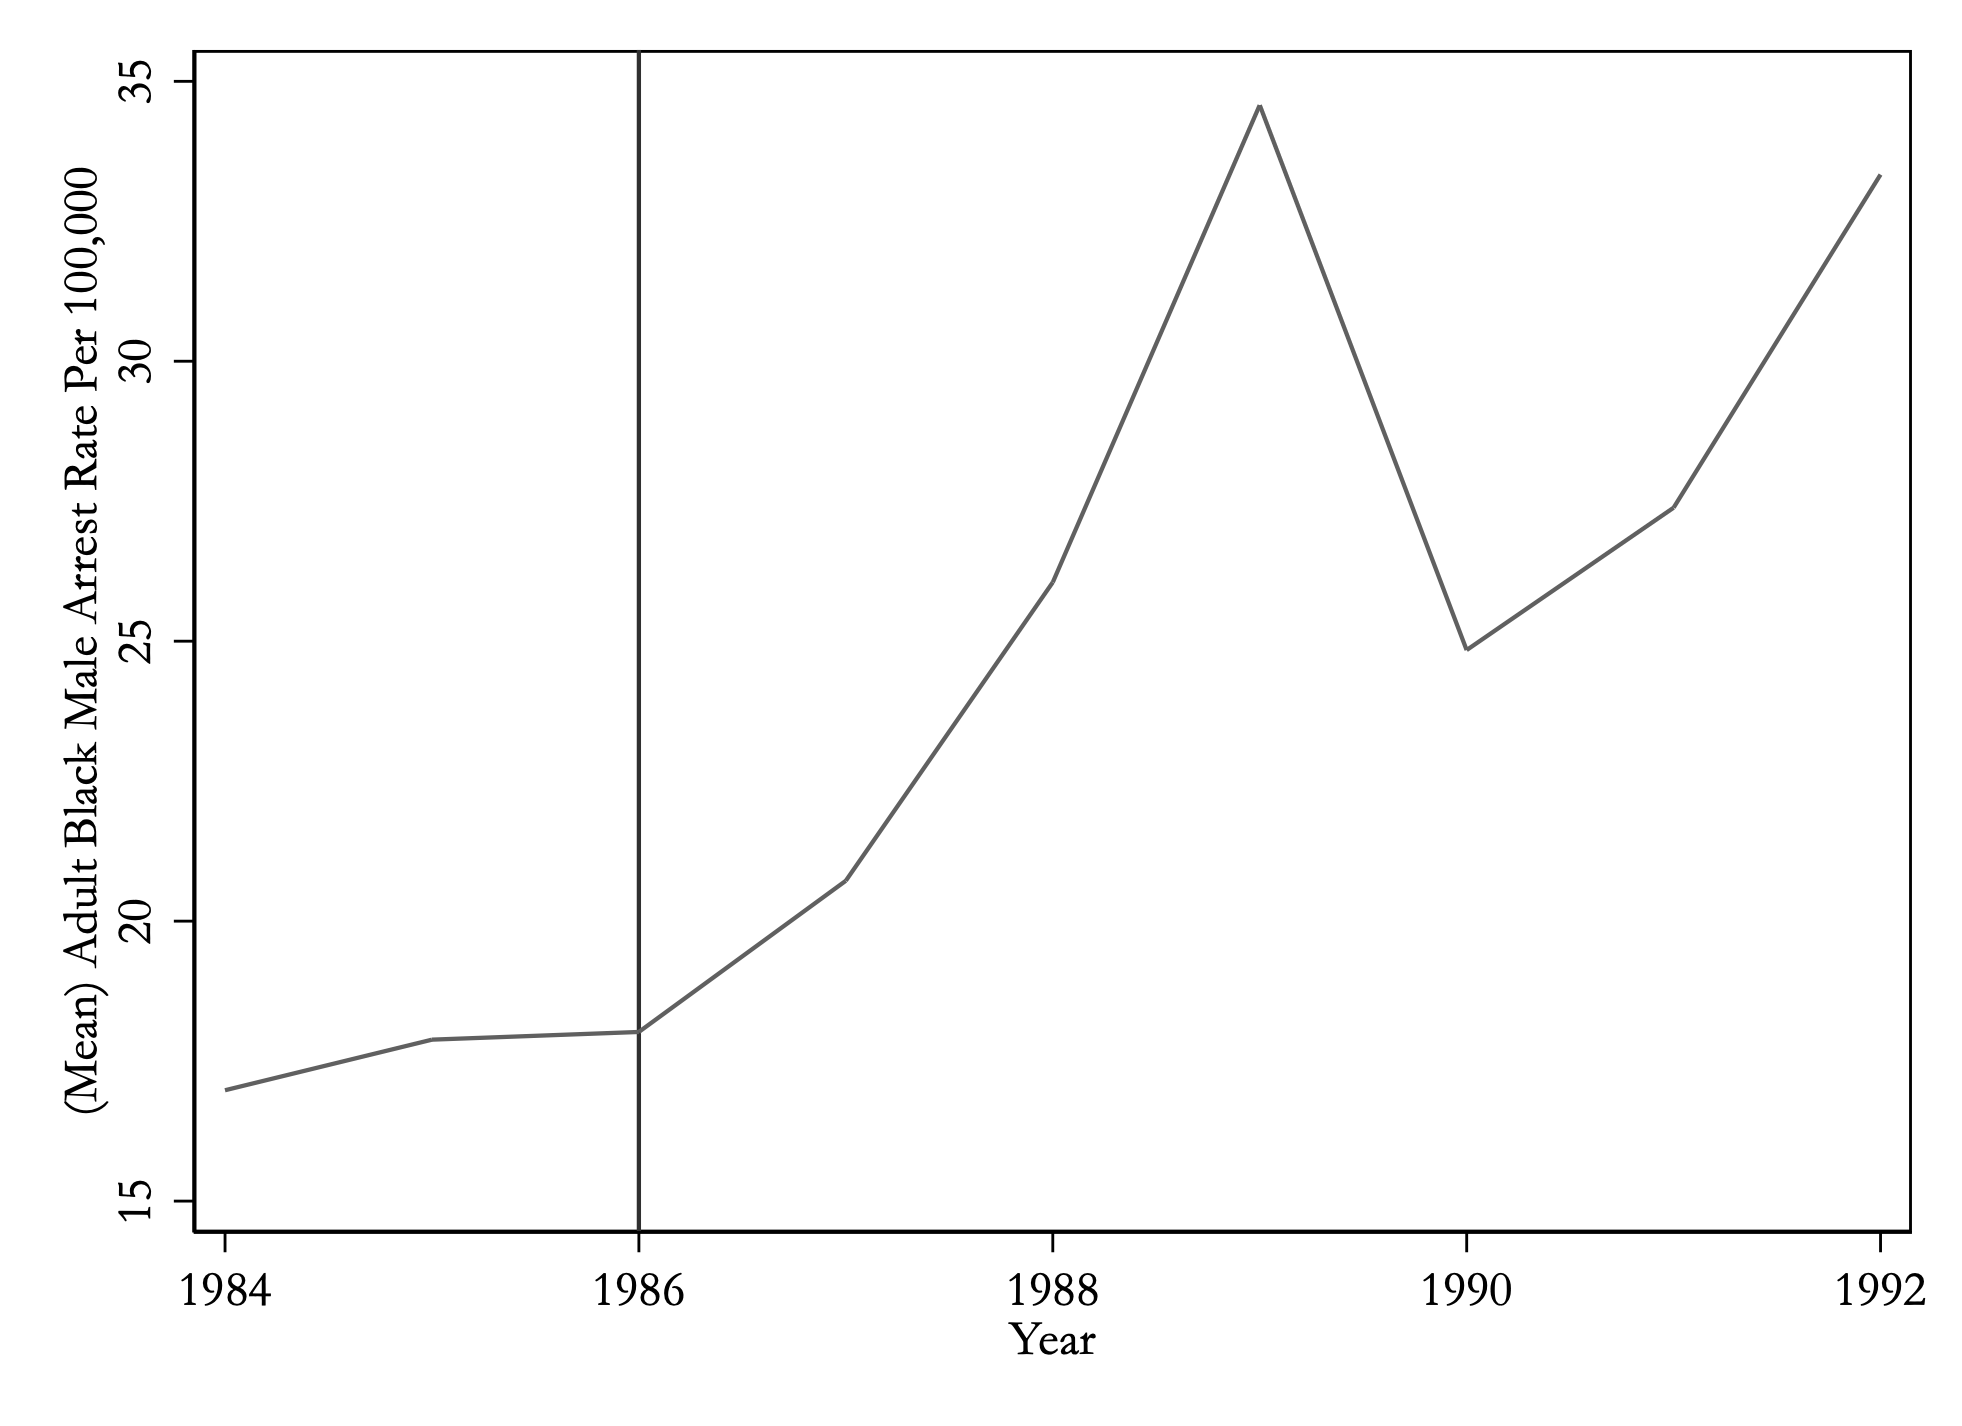
\includegraphics[width=7cm]{pretrends/1986/ab.png} }}%
    \qquad
    \subfloat[\centering 2010]{{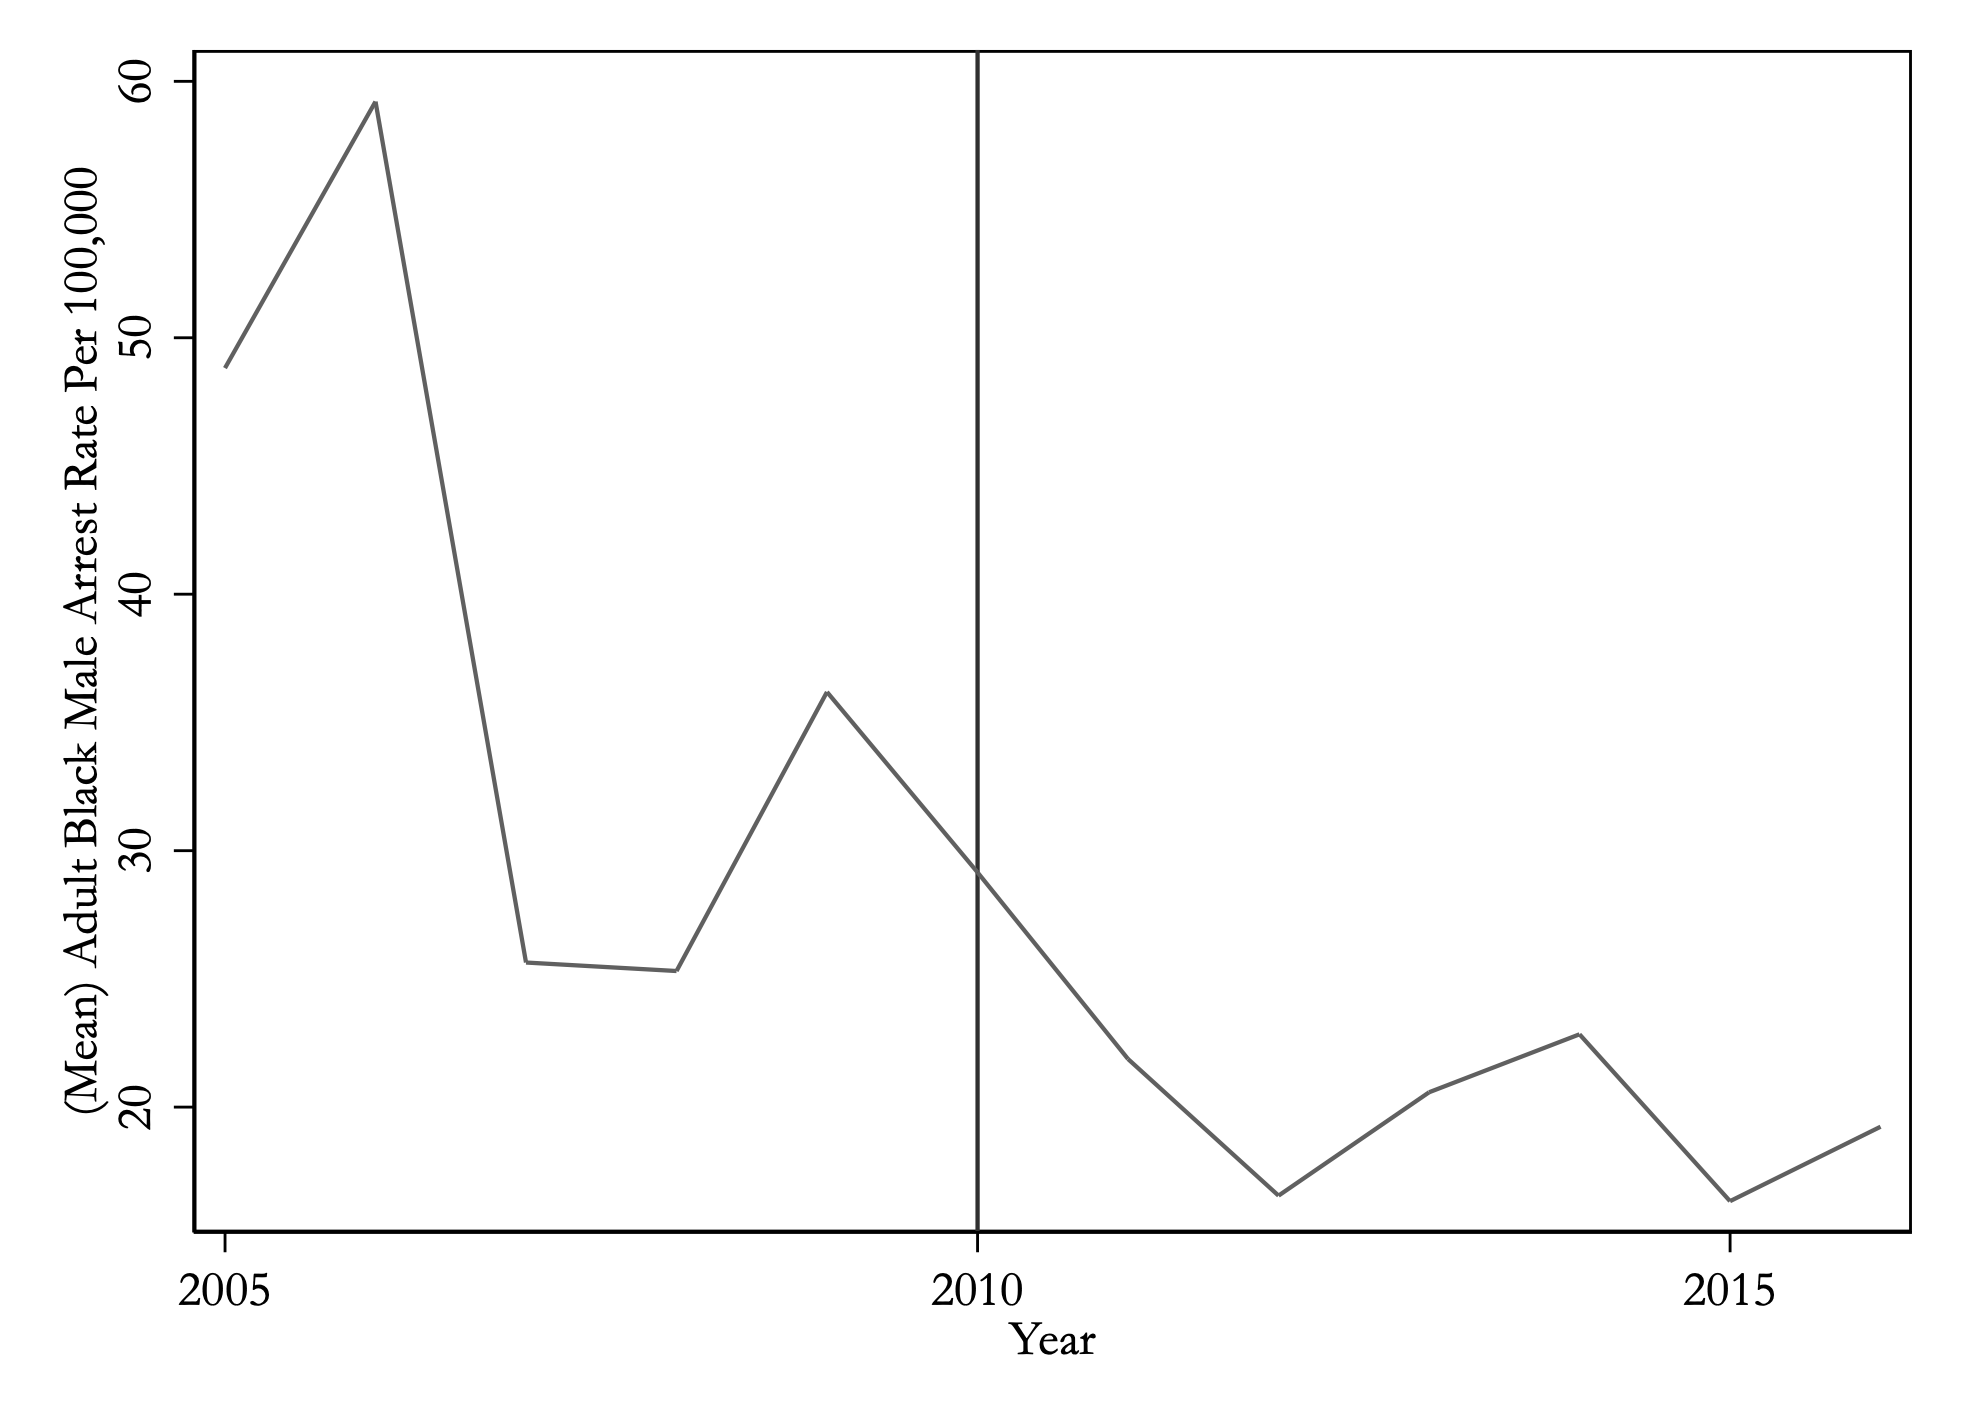
\includegraphics[width=7cm]{pretrends/2010/ab.png} }}%
    \label{fig:raw_ab}%
  \end{figure}
  \begin{figure}[h]
    \centering
    \caption{Juvenile Black Arrest Rate Per 100,000}%
    \subfloat[\centering 1986]{{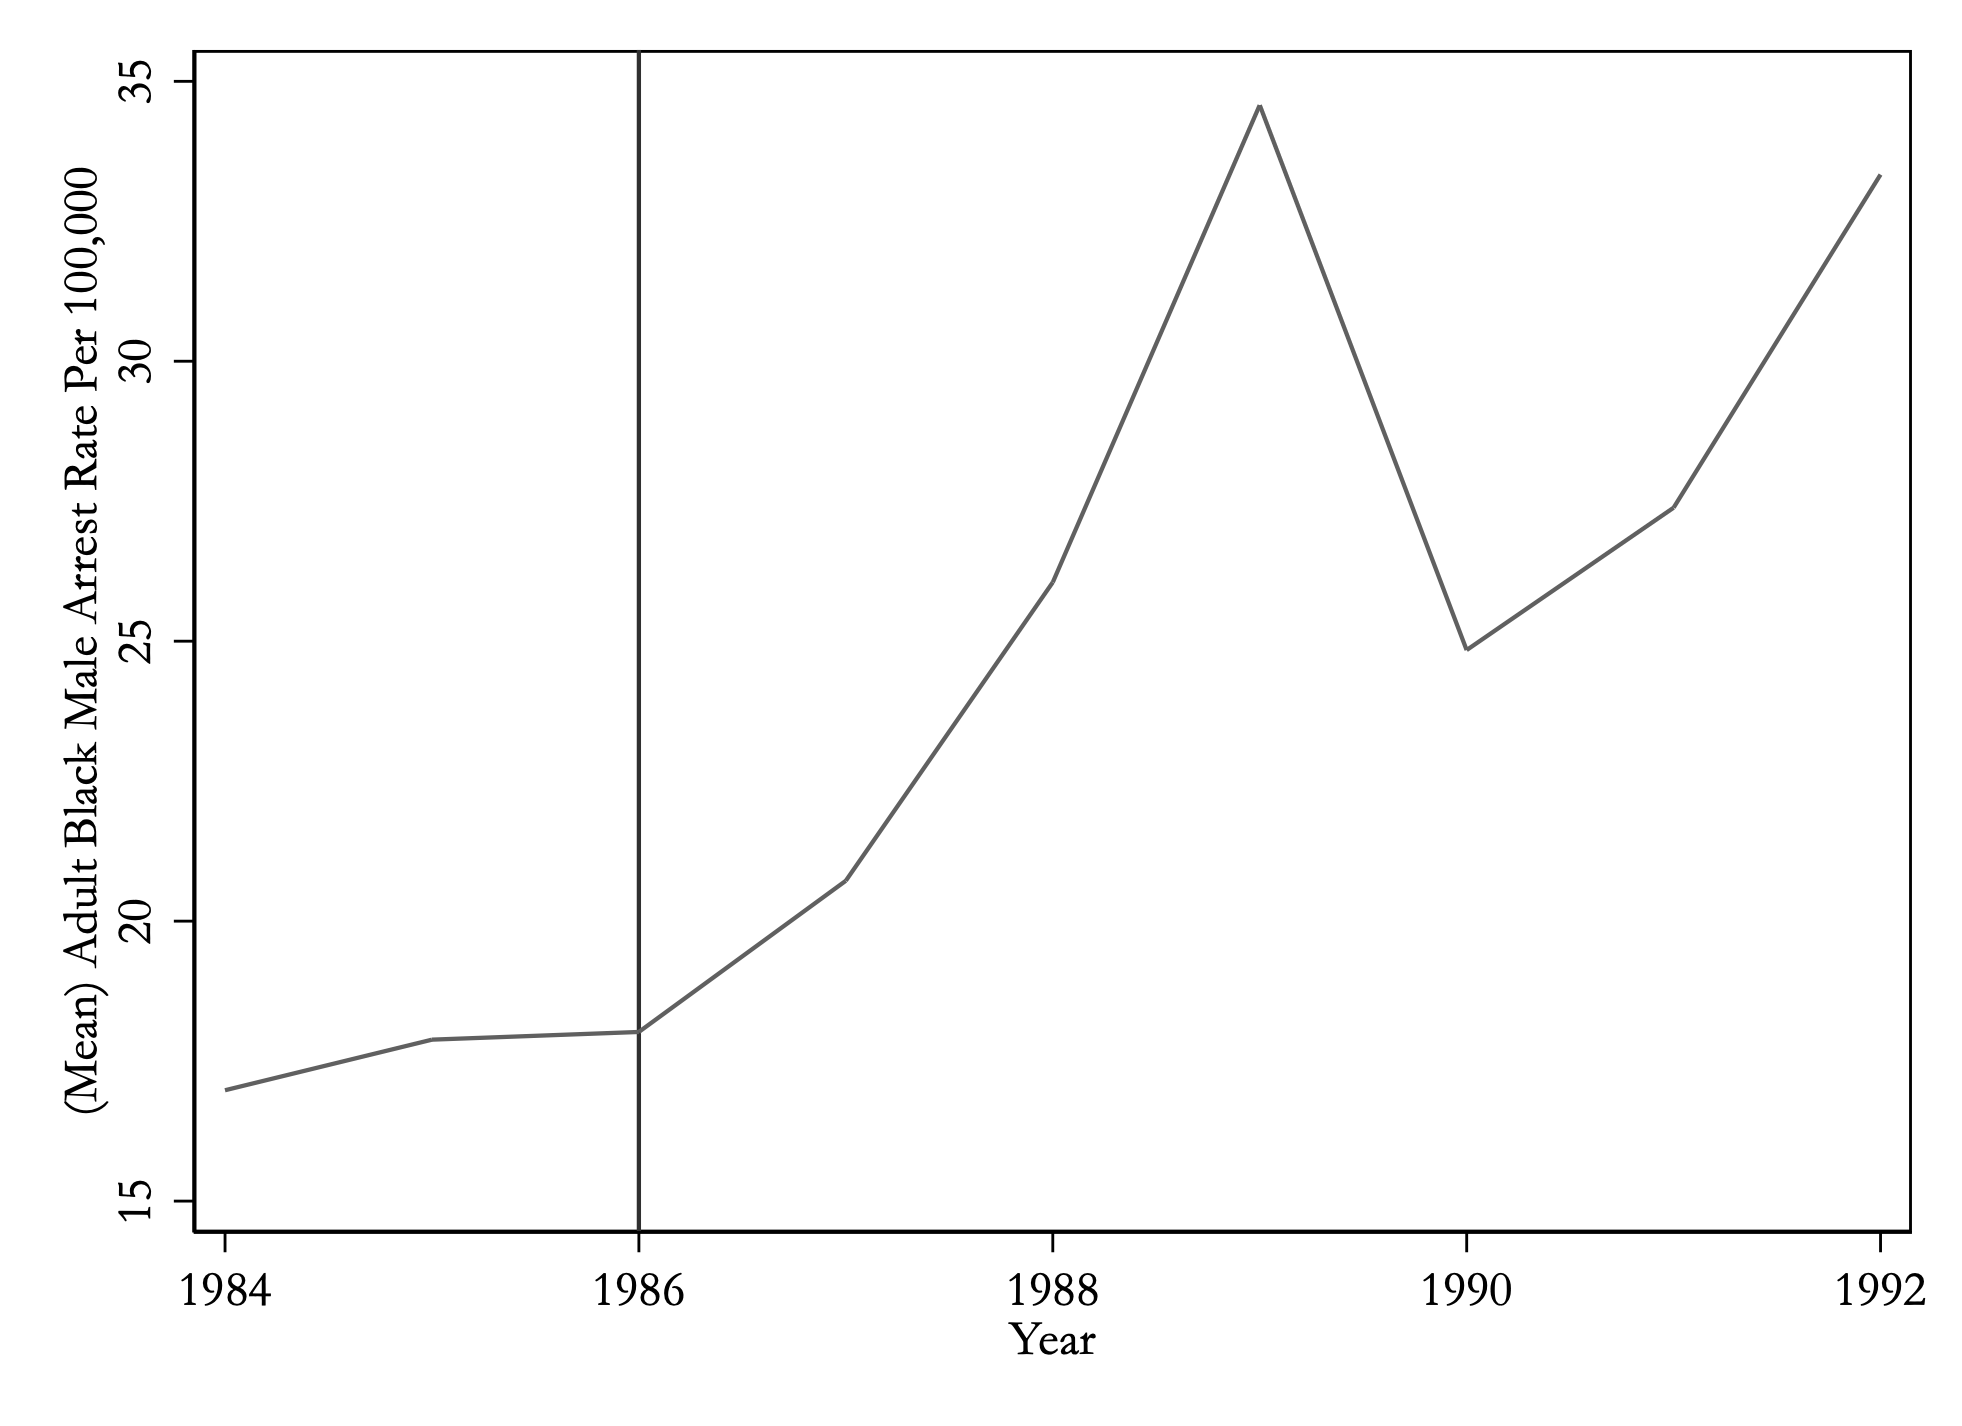
\includegraphics[width=7cm]{pretrends/1986/ab.png} }}%
    \qquad
    \subfloat[\centering 2010]{{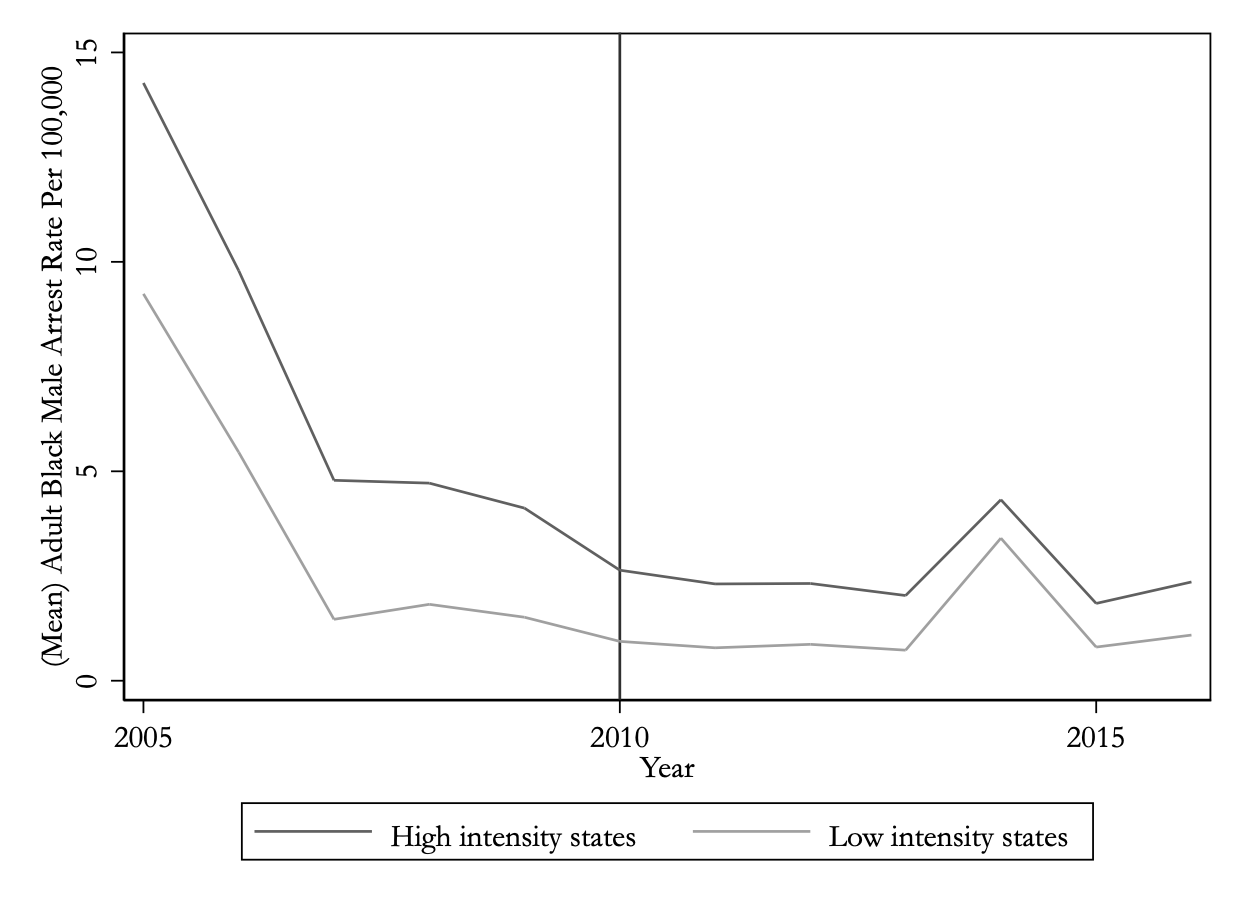
\includegraphics[width=7cm]{pretrends/2010/jb.png} }}%
    \label{fig:raw_jb}%
  \end{figure}

  \begin{footnotesize}
    \noindent Note: These figures report the drug crime arrest rate per 100,000 for black adults and black juveniles separately over time using CPS-UCR merged data from 1984-1992 and 2005-2016. A vertical line is drawn to denote the passage of the Anti-Drug Abuse Act of 1986 and the Fair Sentencing Act of 2010.
  \end{footnotesize}
  
  \clearpage
  
  % High vs low arrest states pre-trends

  \begin{figure}[h]
    \centering
    \caption{College Enrollment By States with High vs Low Black Adult Drug Arrest Rates}%
    \subfloat[\centering 1986]{{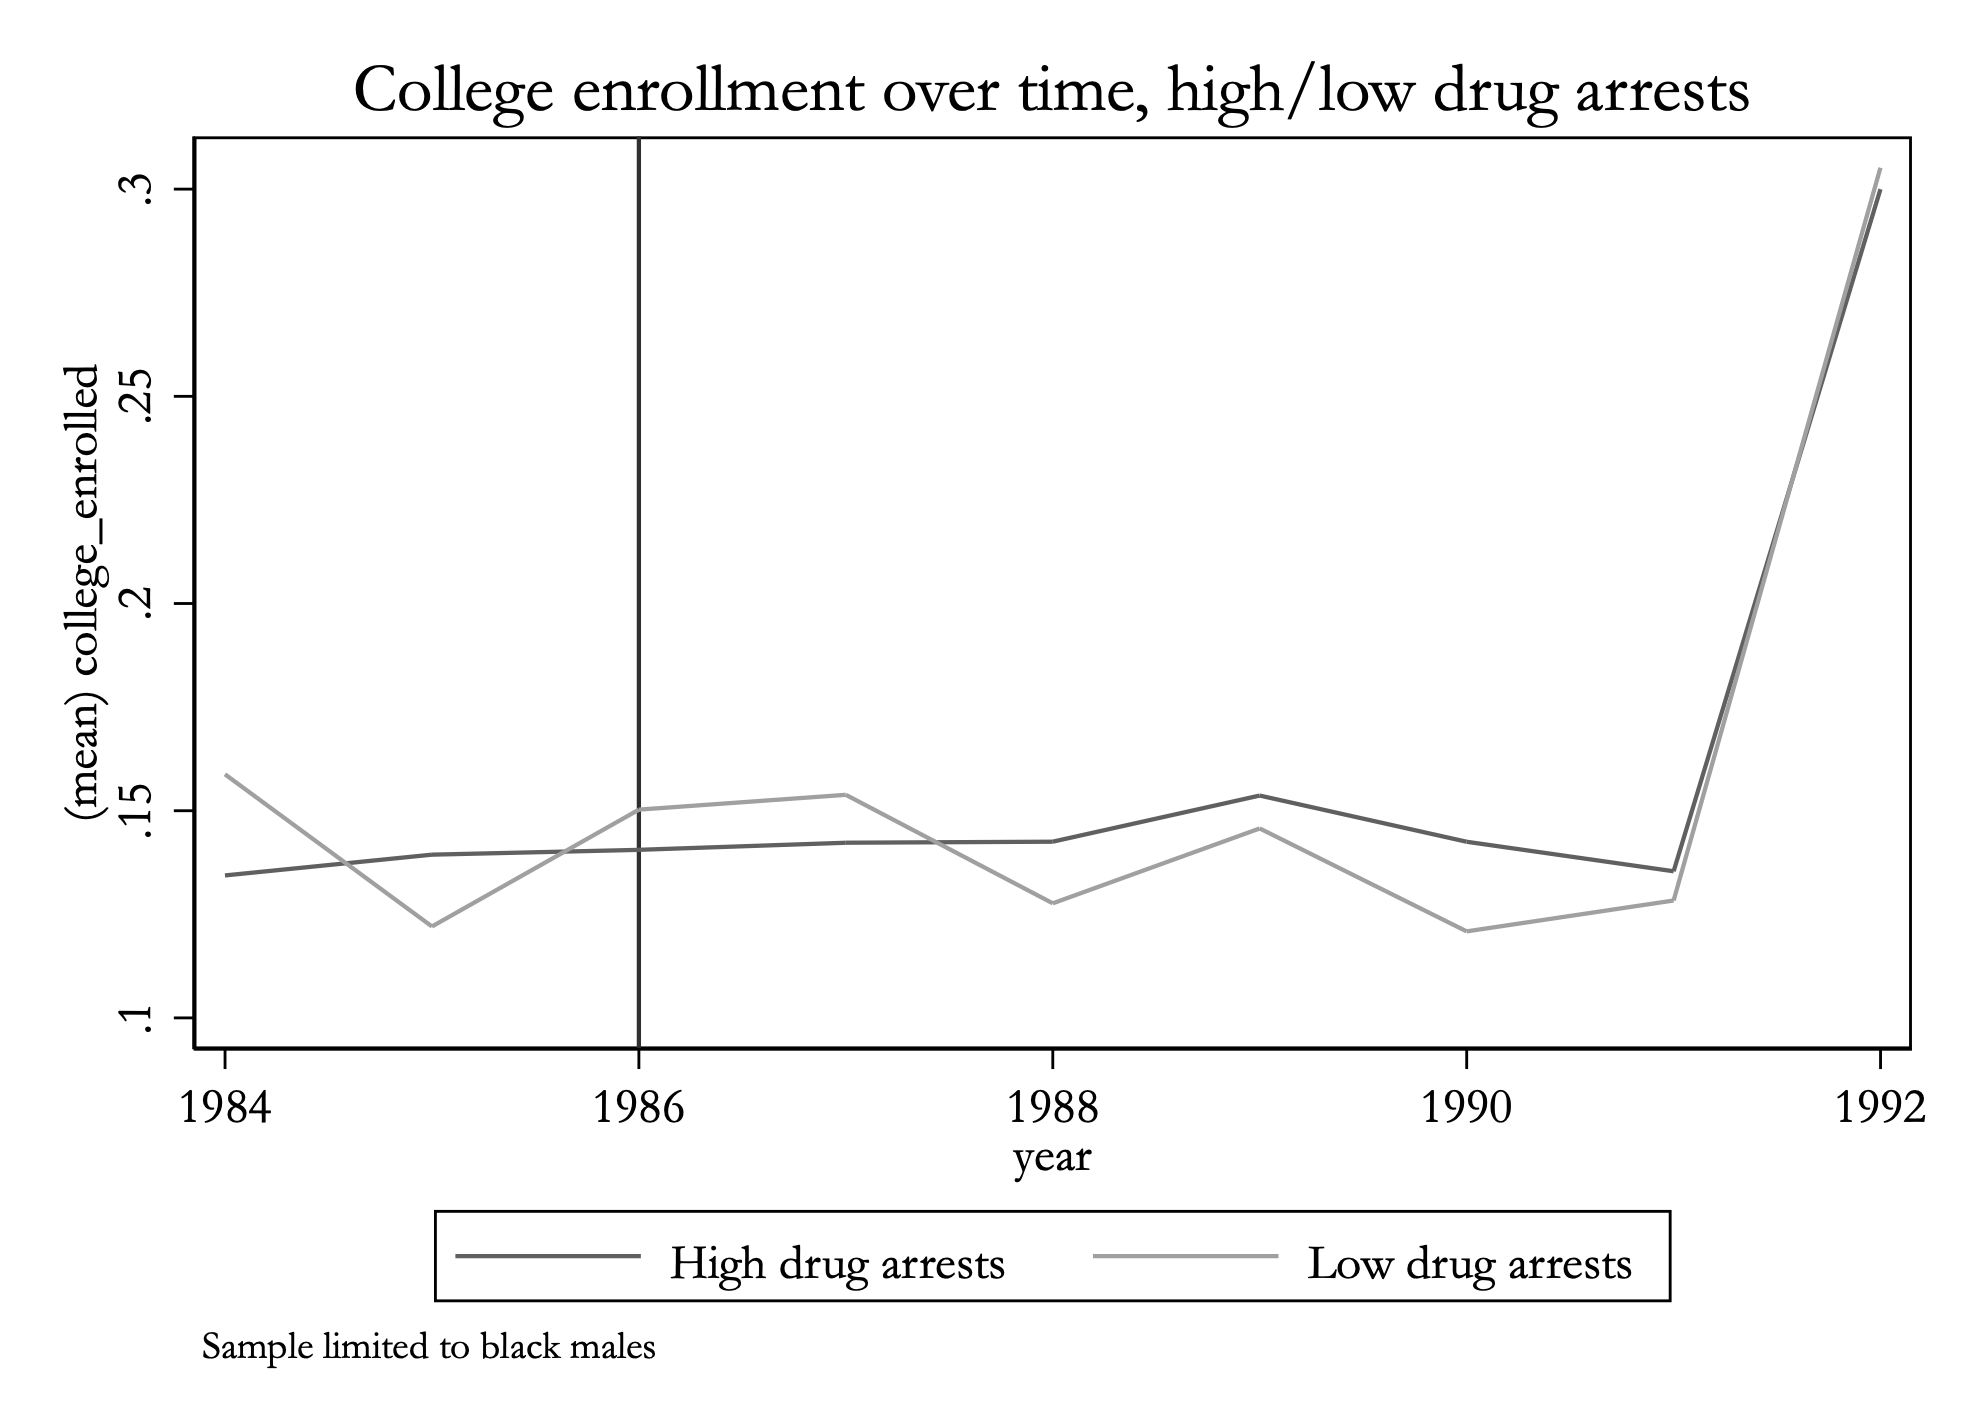
\includegraphics[width=7cm]{pretrends/1986/college_enroll_bydrugarrests_1986.png} }}%
    \qquad
    \subfloat[\centering 2010]{{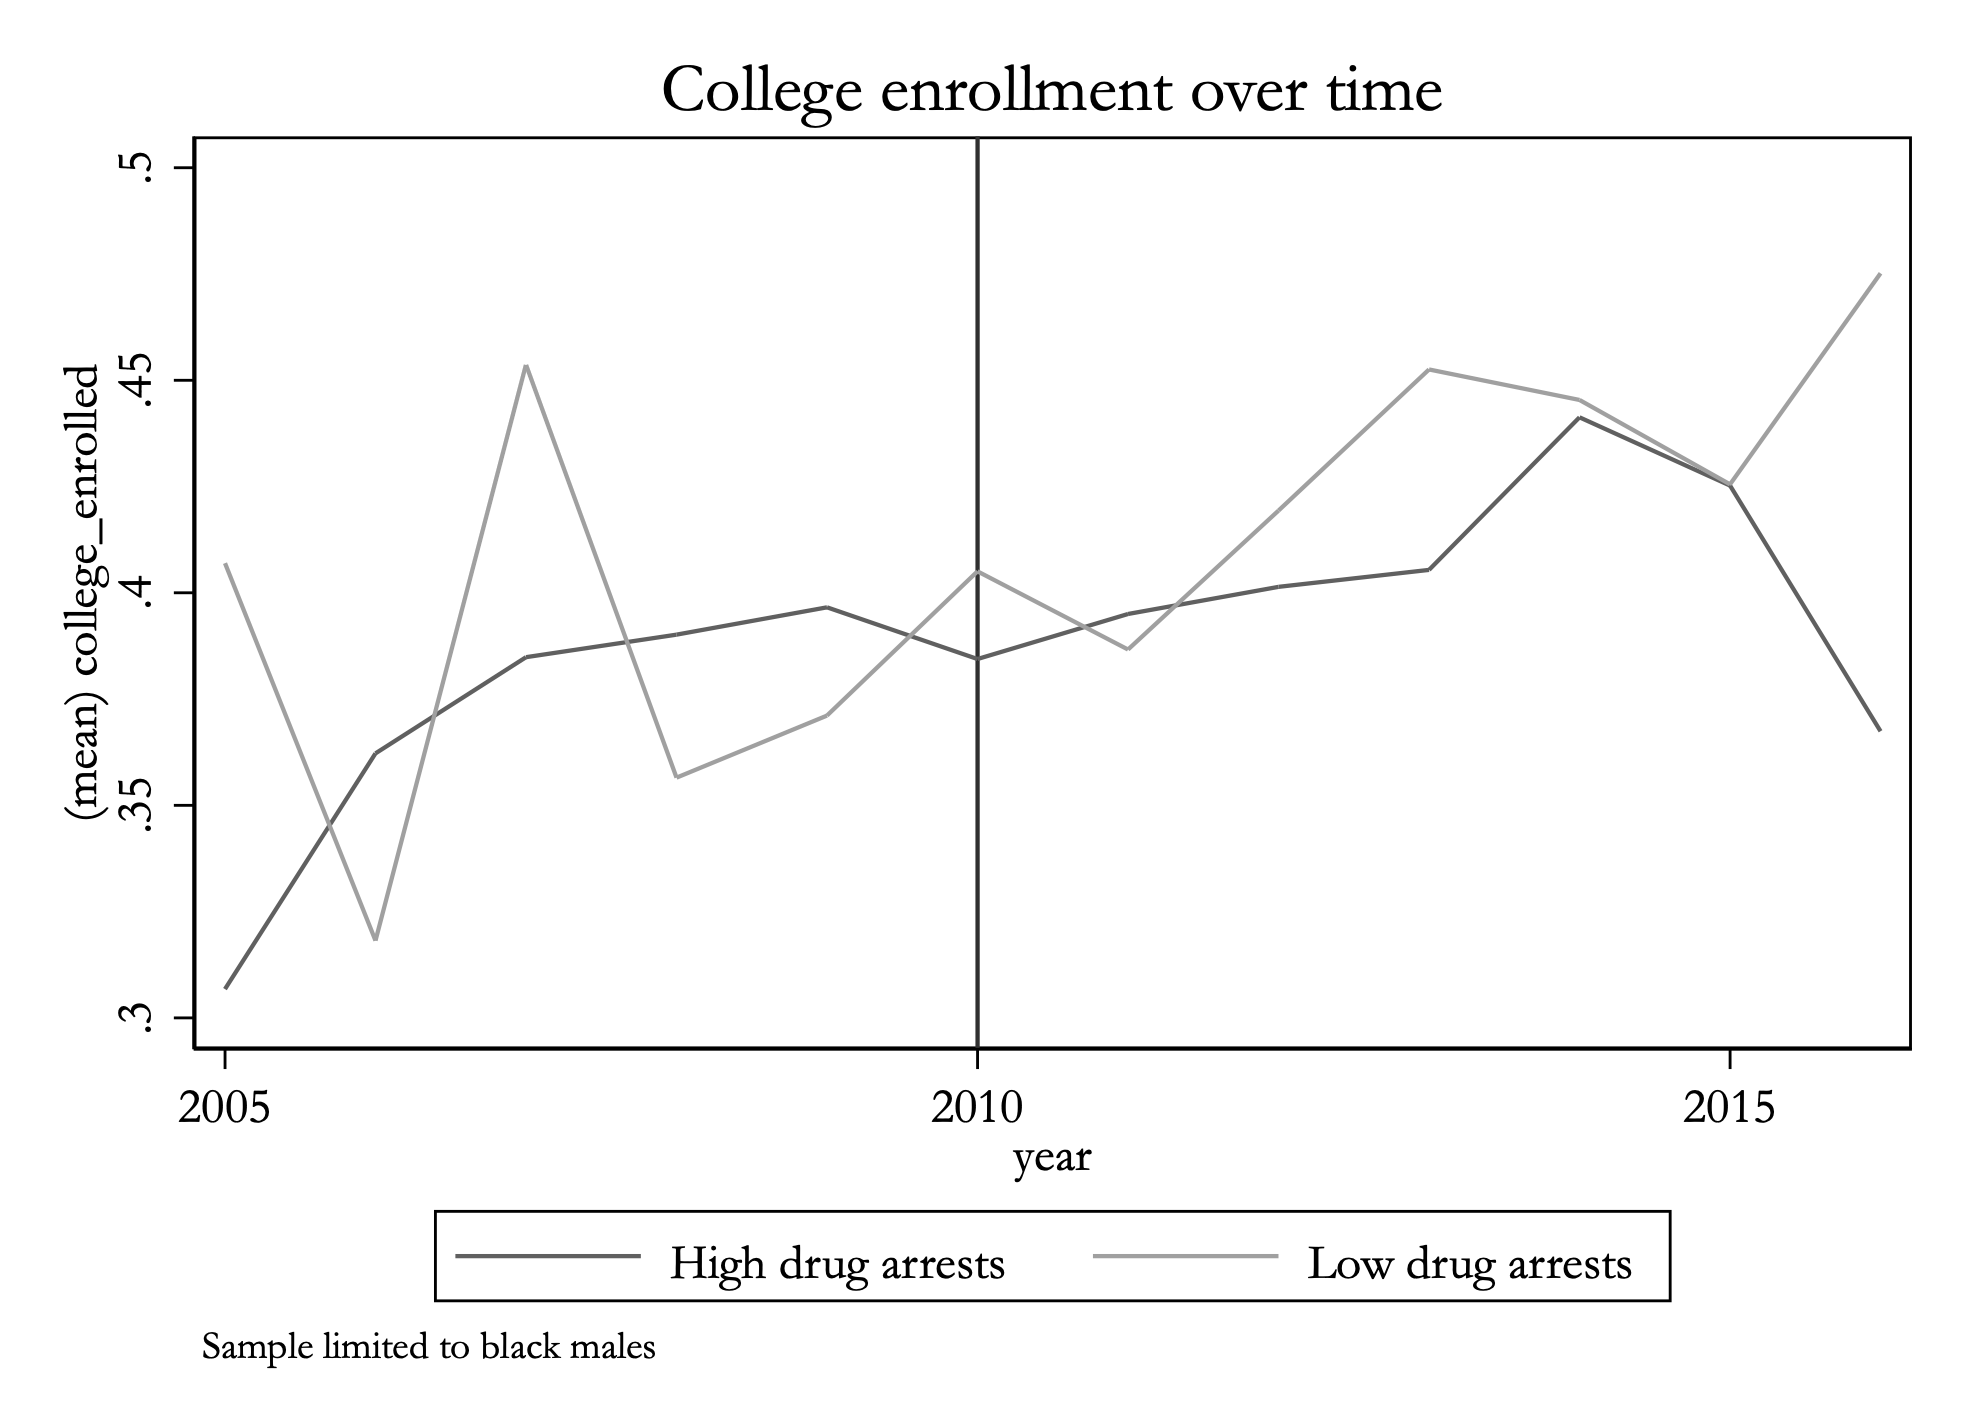
\includegraphics[width=7cm]{pretrends/2010/college_enroll_bydrugarrests_2010.png} }}%
    \label{fig:raw_college_highlowab_1986}%
  \end{figure}
  \begin{figure}[h]
    \centering
    \caption{College Enrollment By States with High vs Low Black Juvenile Drug Arrest Rates}%
    \subfloat[\centering 1986]{{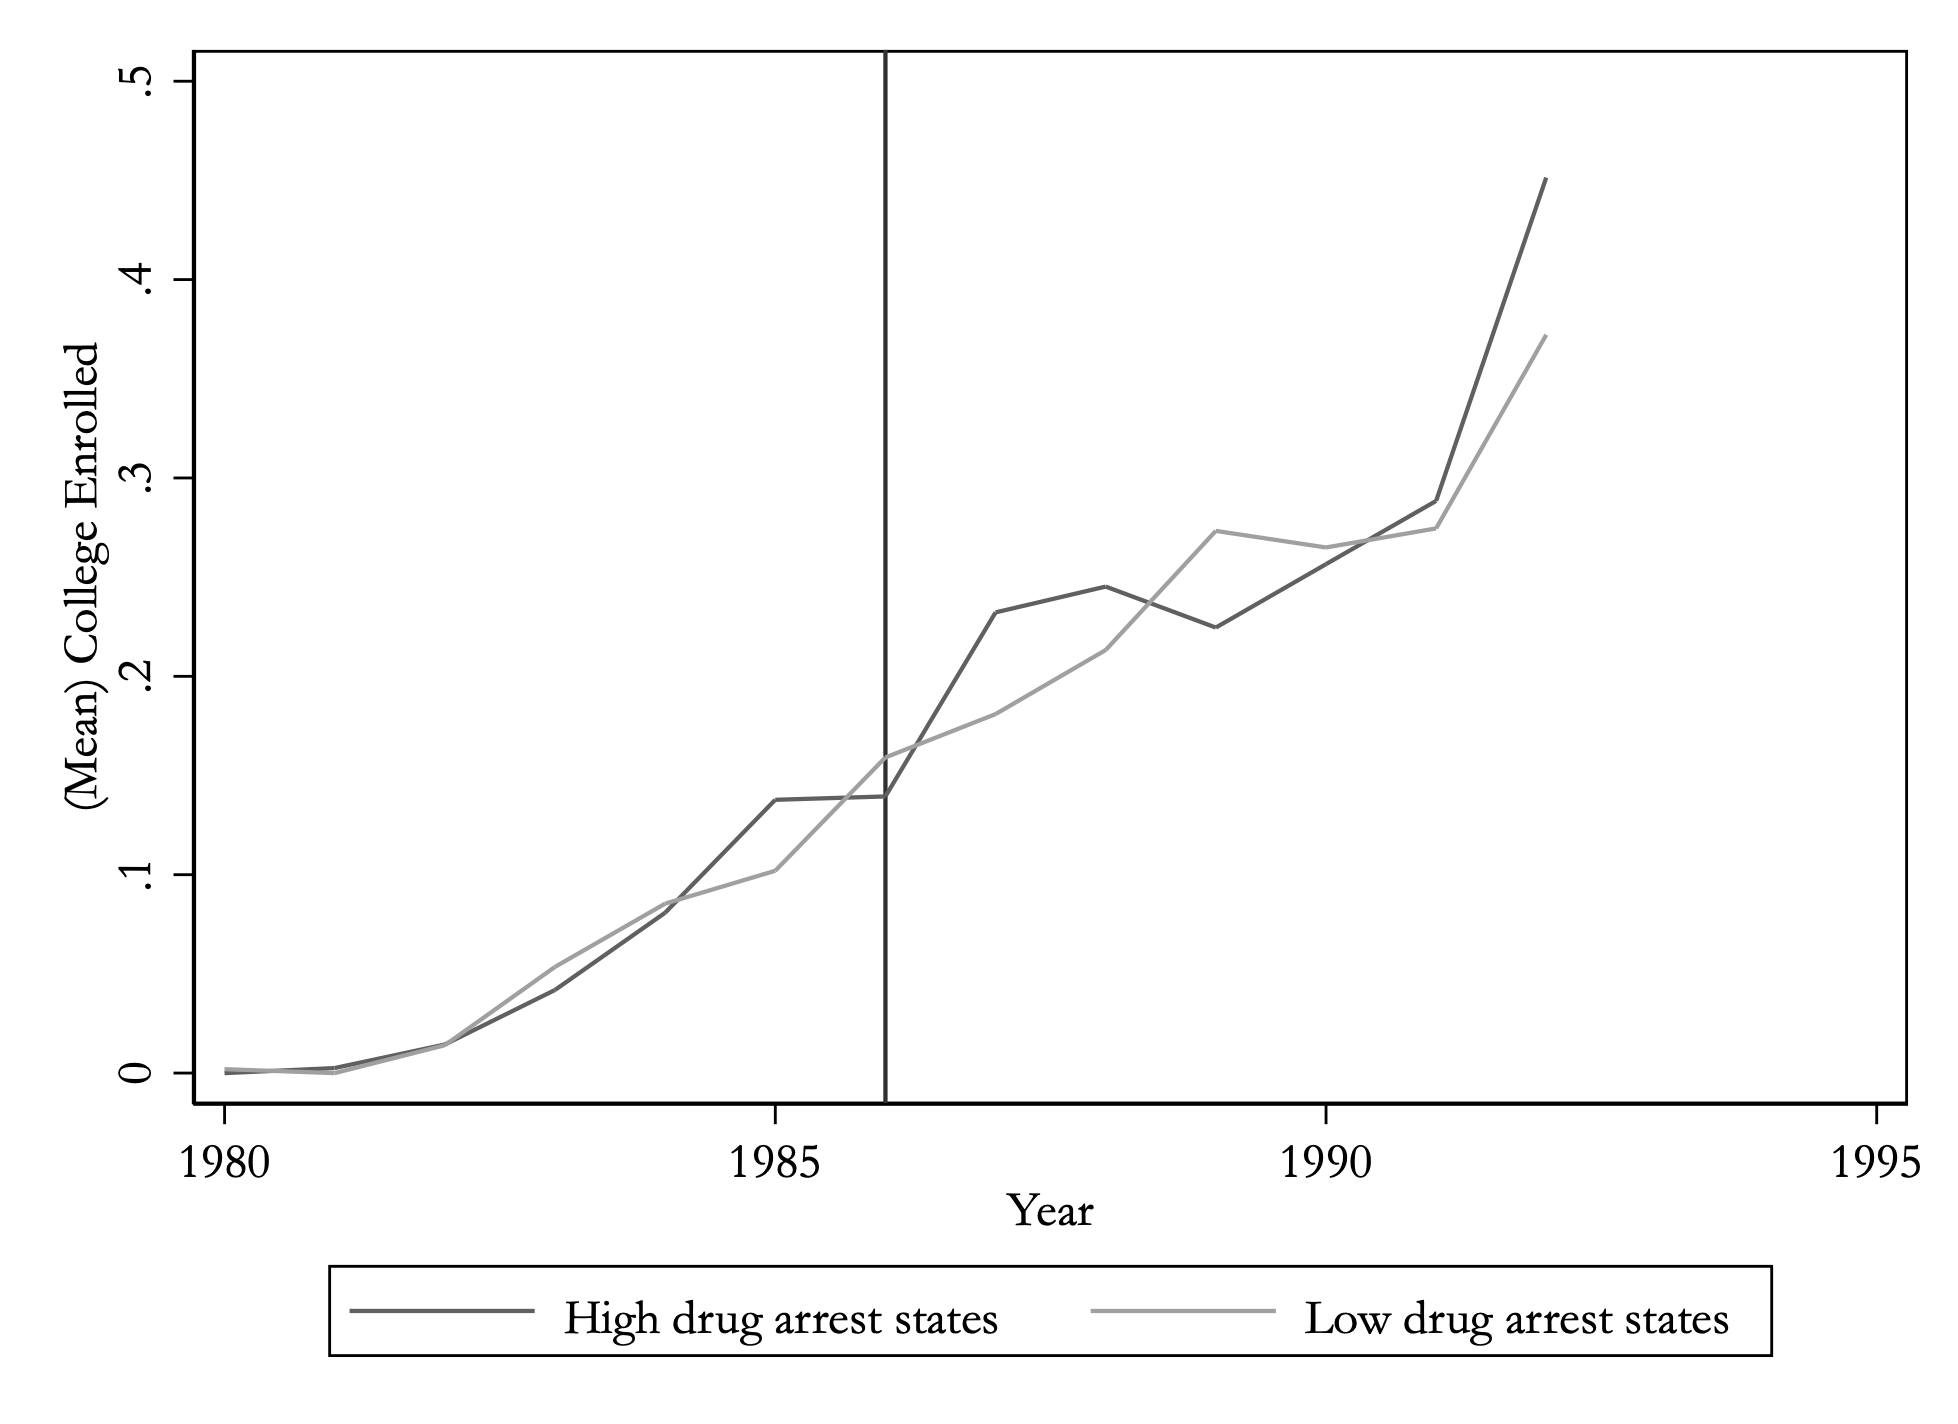
\includegraphics[width=7cm]{pretrends/1986/college_enroll_bydrugarrests_jb_1986.png} }}%
    \qquad
    \subfloat[\centering 2010]{{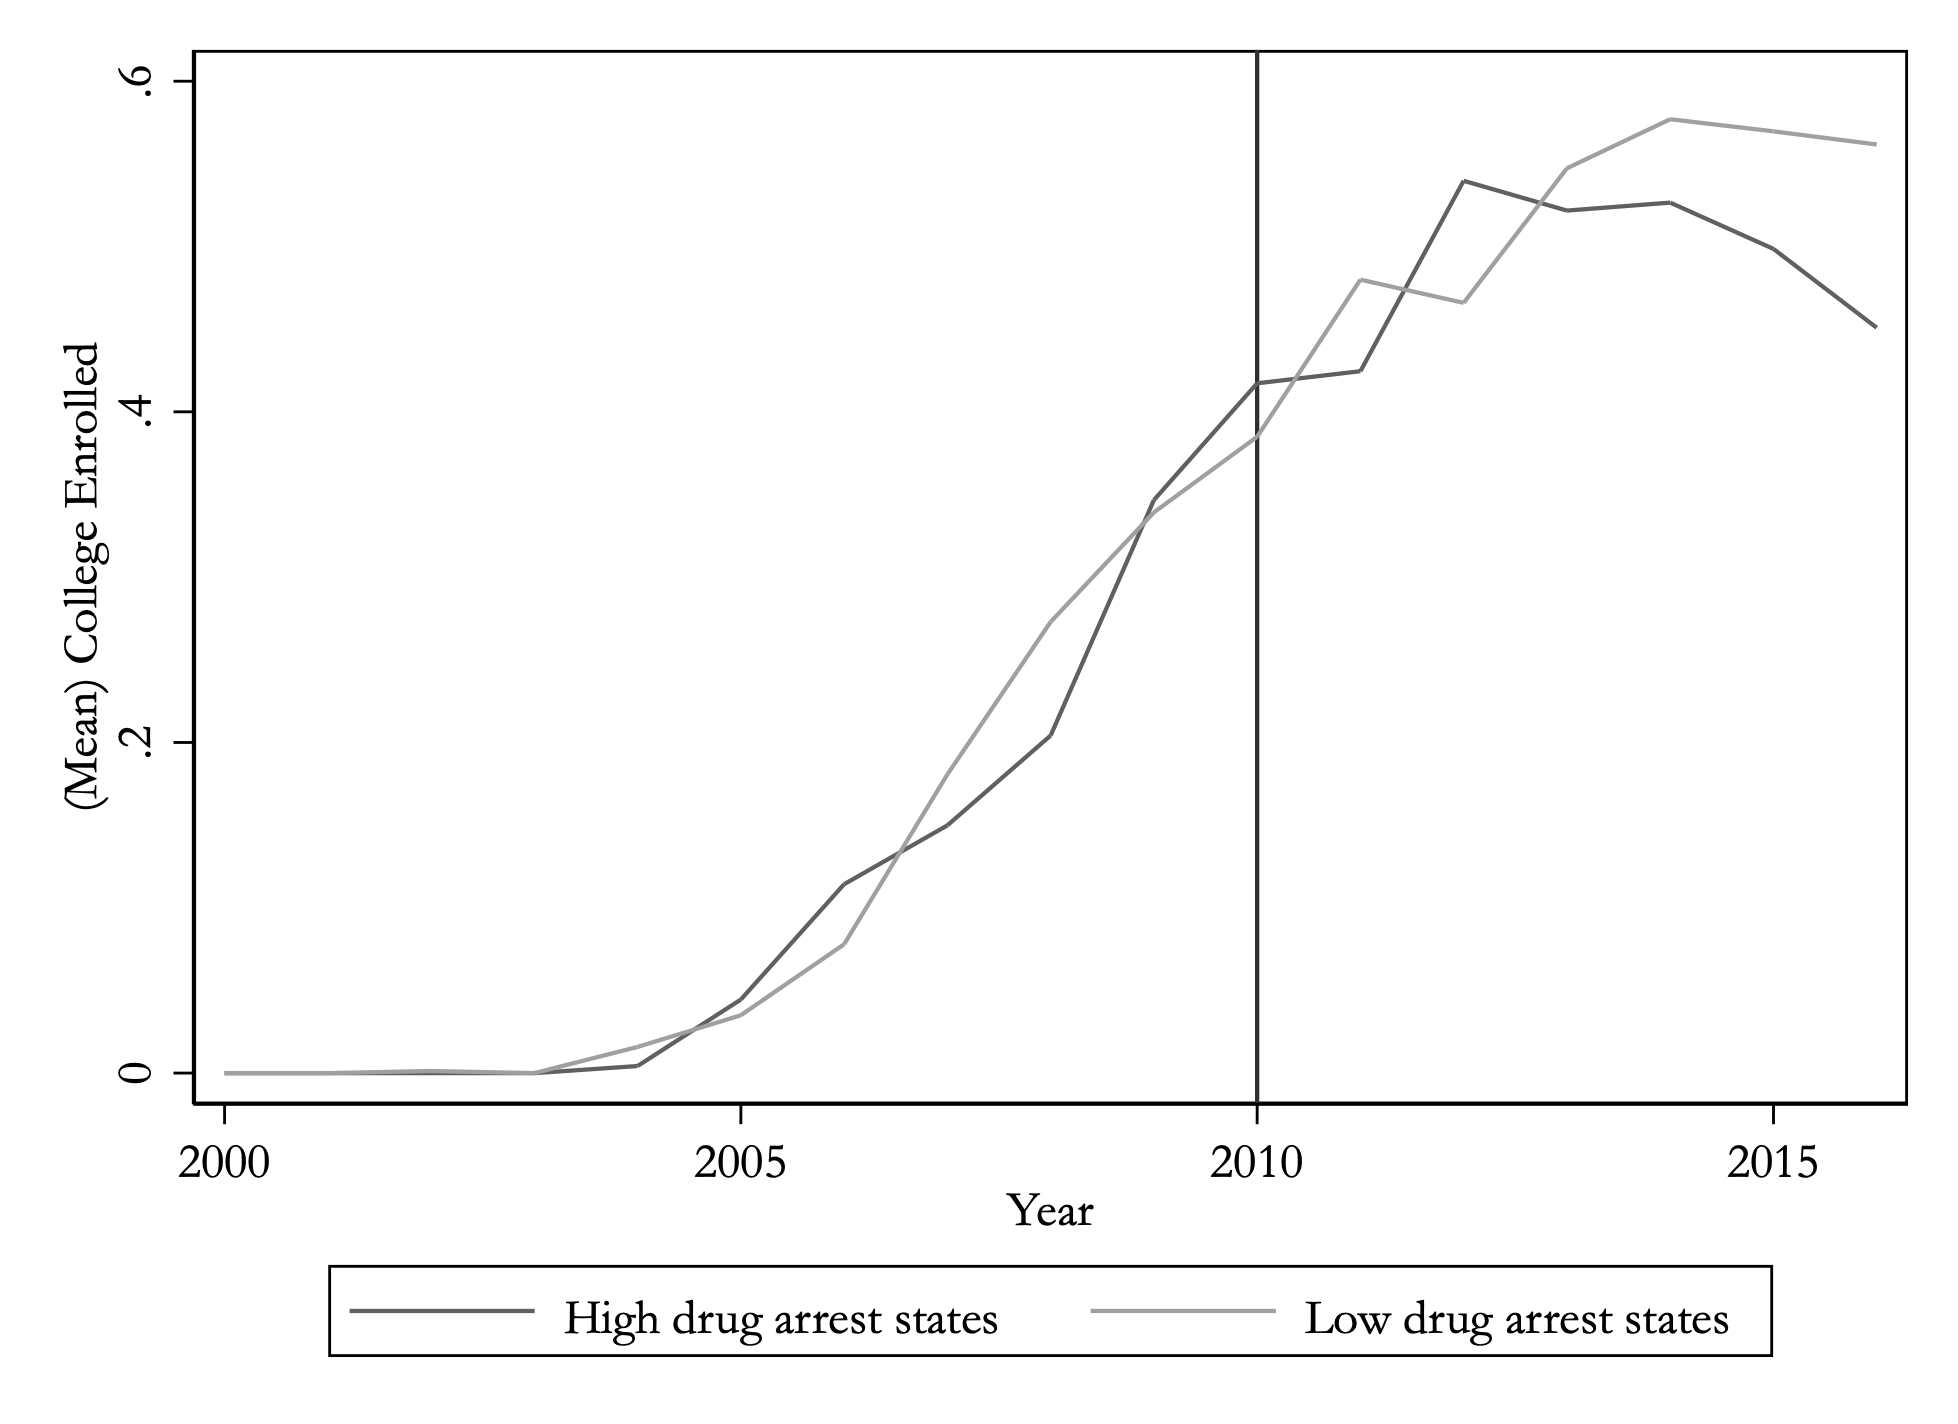
\includegraphics[width=7cm]{pretrends/2010/college_enroll_bydrugarrests_jb_2010.png} }}%
    \label{fig:raw_college_highlowjb_1986}%
  \end{figure}
  
  \begin{footnotesize}
    \noindent Note: These figures report the proportion enrolled in college plotted over time using CPS data from 1984-1992 and 2005-2016 for high black adult/juvenile drug arrest states and low black adult/juvenile drug arrest states, where high black adult/juvenile drug arrest states are defined to be those above the 75th percentile in 1984 and 2008. A vertical line is drawn to denote the passage of the Anti-Drug Abuse Act of 1986 and the Fair Sentencing Act of 2010. The sample is defined as black males aged 18-24 in 1986 and 2010 who were not incarcerated at the time of the survey.
  \end{footnotesize}
  
  \clearpage

  \begin{figure}[h]
    \caption{Black Adult Drug-related Arrest Rate Per 100,000 in 1984} 
    \centering
    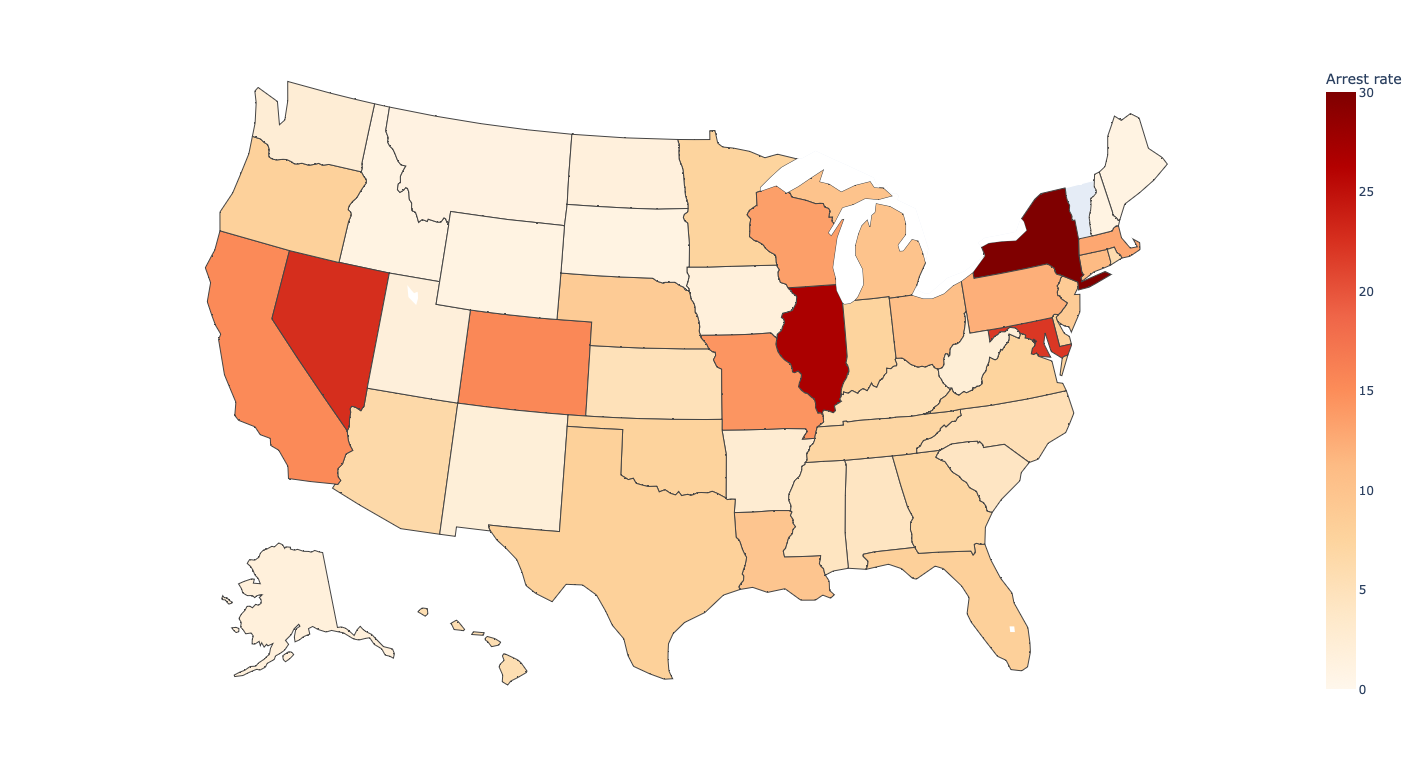
\includegraphics[width=0.8\textwidth]{heatmap/ab1986.png}
    \label{fig:heatmap}
  \end{figure}
  
  \begin{footnotesize}
    \noindent Note: This figure presents a heatmap of the United States at the state level using UCR Program data. The data is from 1984, and I use all drug-related arrests for Black adult men. Although New York's normalized arrest rate is at 48, I capped the maximum at 30 for clarity of states with low normalized drug arrest rates, since the distribution is heavily right-skewed. High drug arrest states are defined as states above the 75th percentile, and the 75th percentile is at 17.4 Black adult arrests per 100,000.
  \end{footnotesize}
  
  \vspace*{8mm}
  
  \begin{figure}[h]
    \centering
    \caption{Distribution of Black Adult Drug-Related Arrest Rates}%
    \subfloat[\centering 1984]{{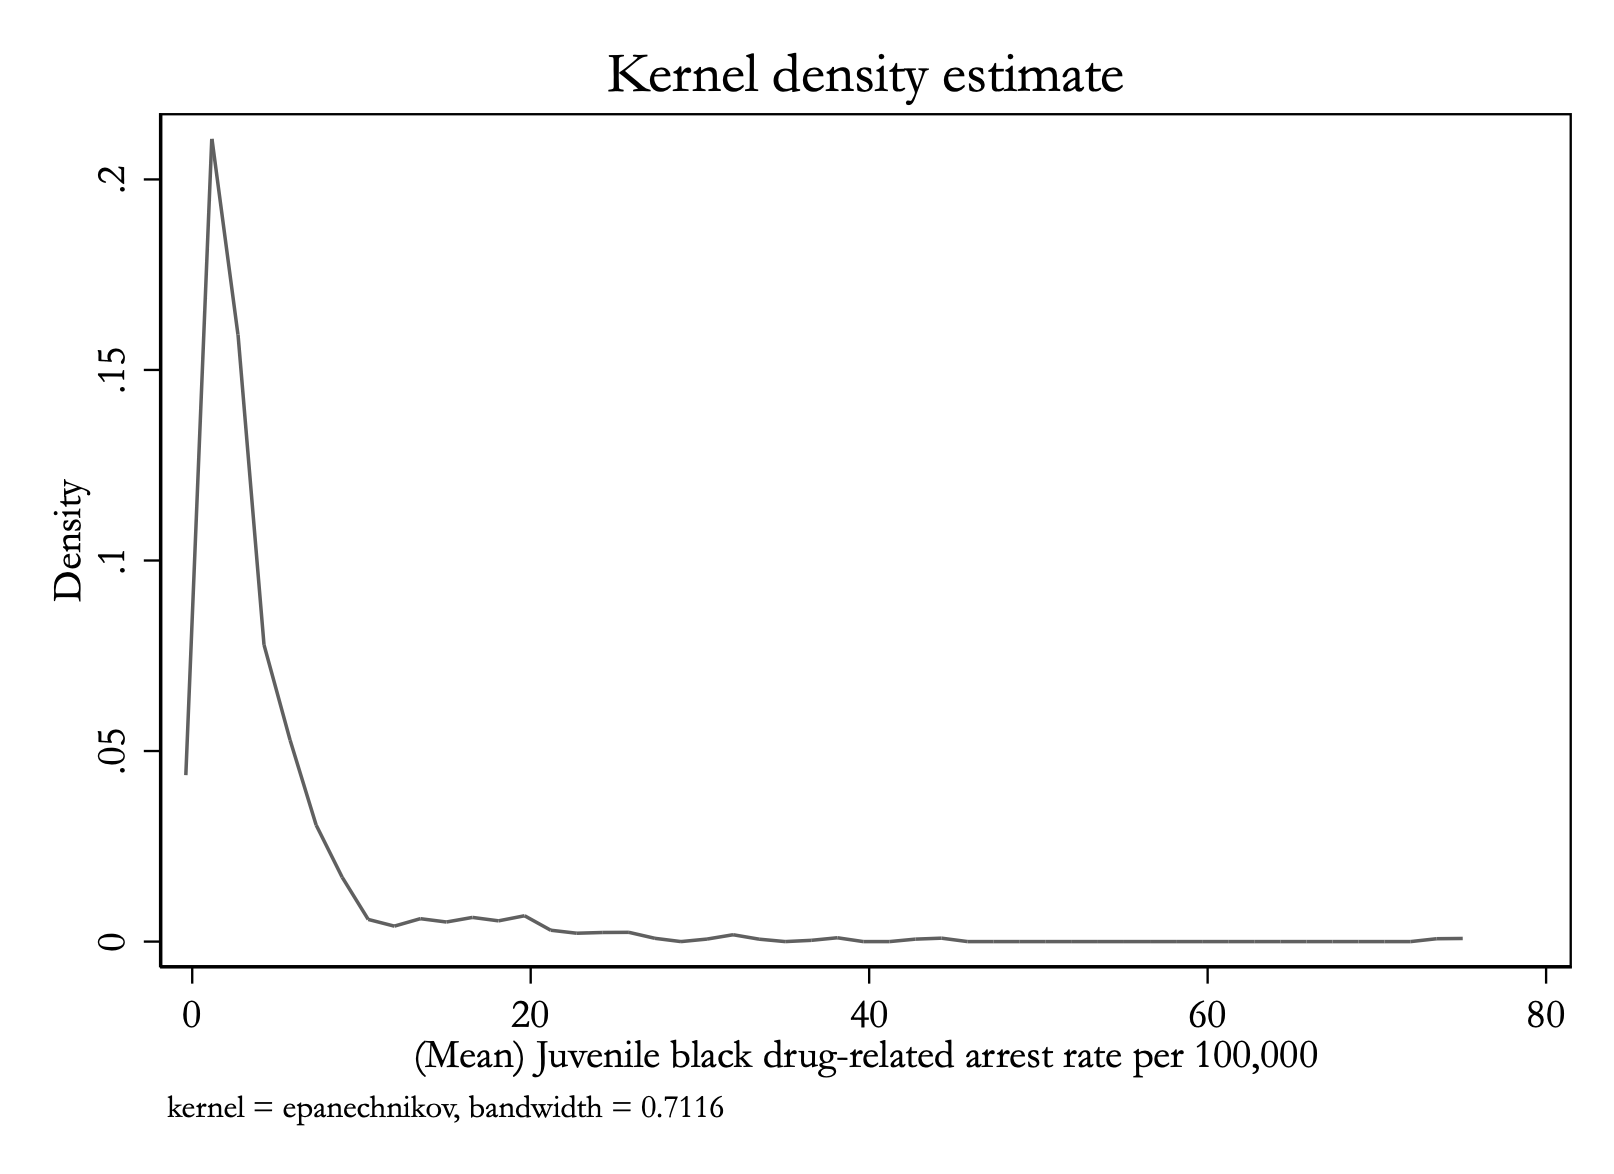
\includegraphics[width=7cm]{descriptive/norm_jb_100000_density_1986} }}%
    \qquad
    \subfloat[\centering 2008]{{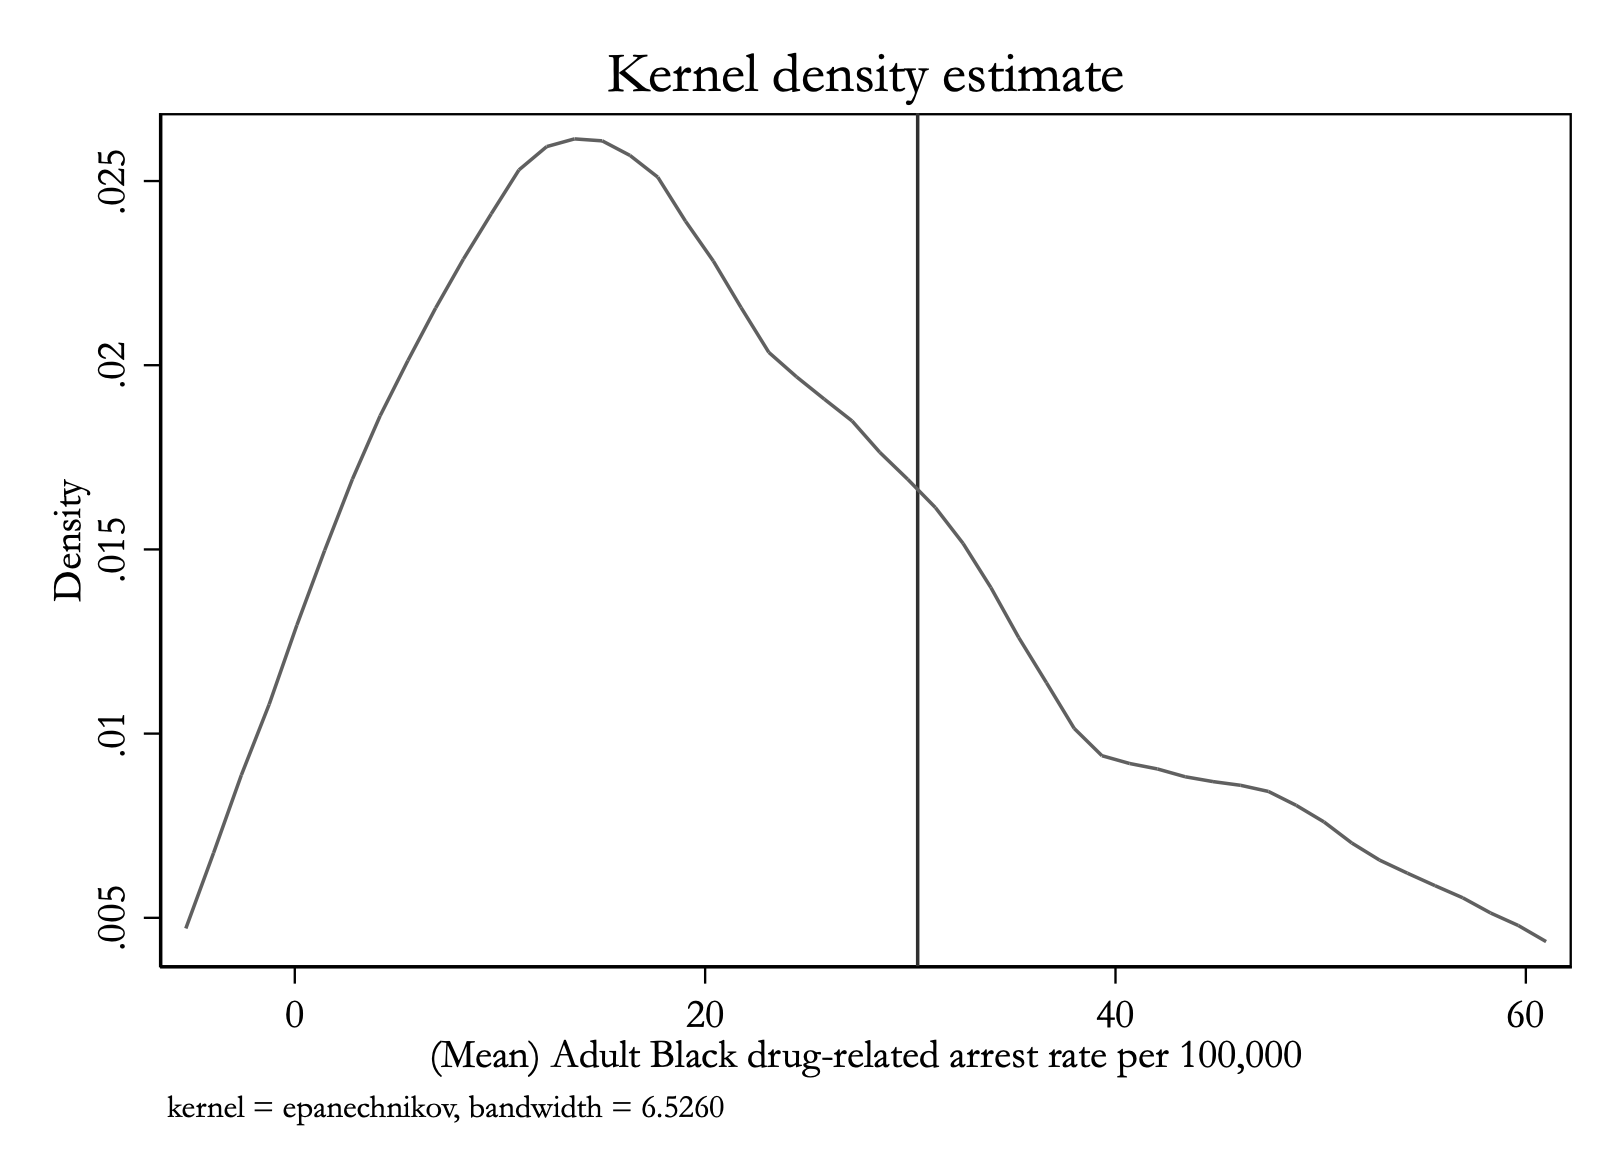
\includegraphics[width=7cm]{descriptive/norm_jb_100000_density_2010.png} }}%
    \label{fig:density_jb}%
  \end{figure}
  \begin{footnotesize}
    \noindent Note: These figures report the kernel density estimates for the normalized drug-related Black adult arrest rate in 1984 and 2008. The vertical line denotes the 75th percentile. Right tail outliers were winsorized at the 95\% level for both figures.
  \end{footnotesize}
  
  \clearpage
     

  % Event study
  \begin{figure}[h]
    \caption{Effect of Anti-Drug Abuse Act on Drug-related Arrest Rate of Adult Black Men, Comparing States with High and Low Black Adult Drug-Related Arrest Rates (with Fixed Effects)}
    \centering
    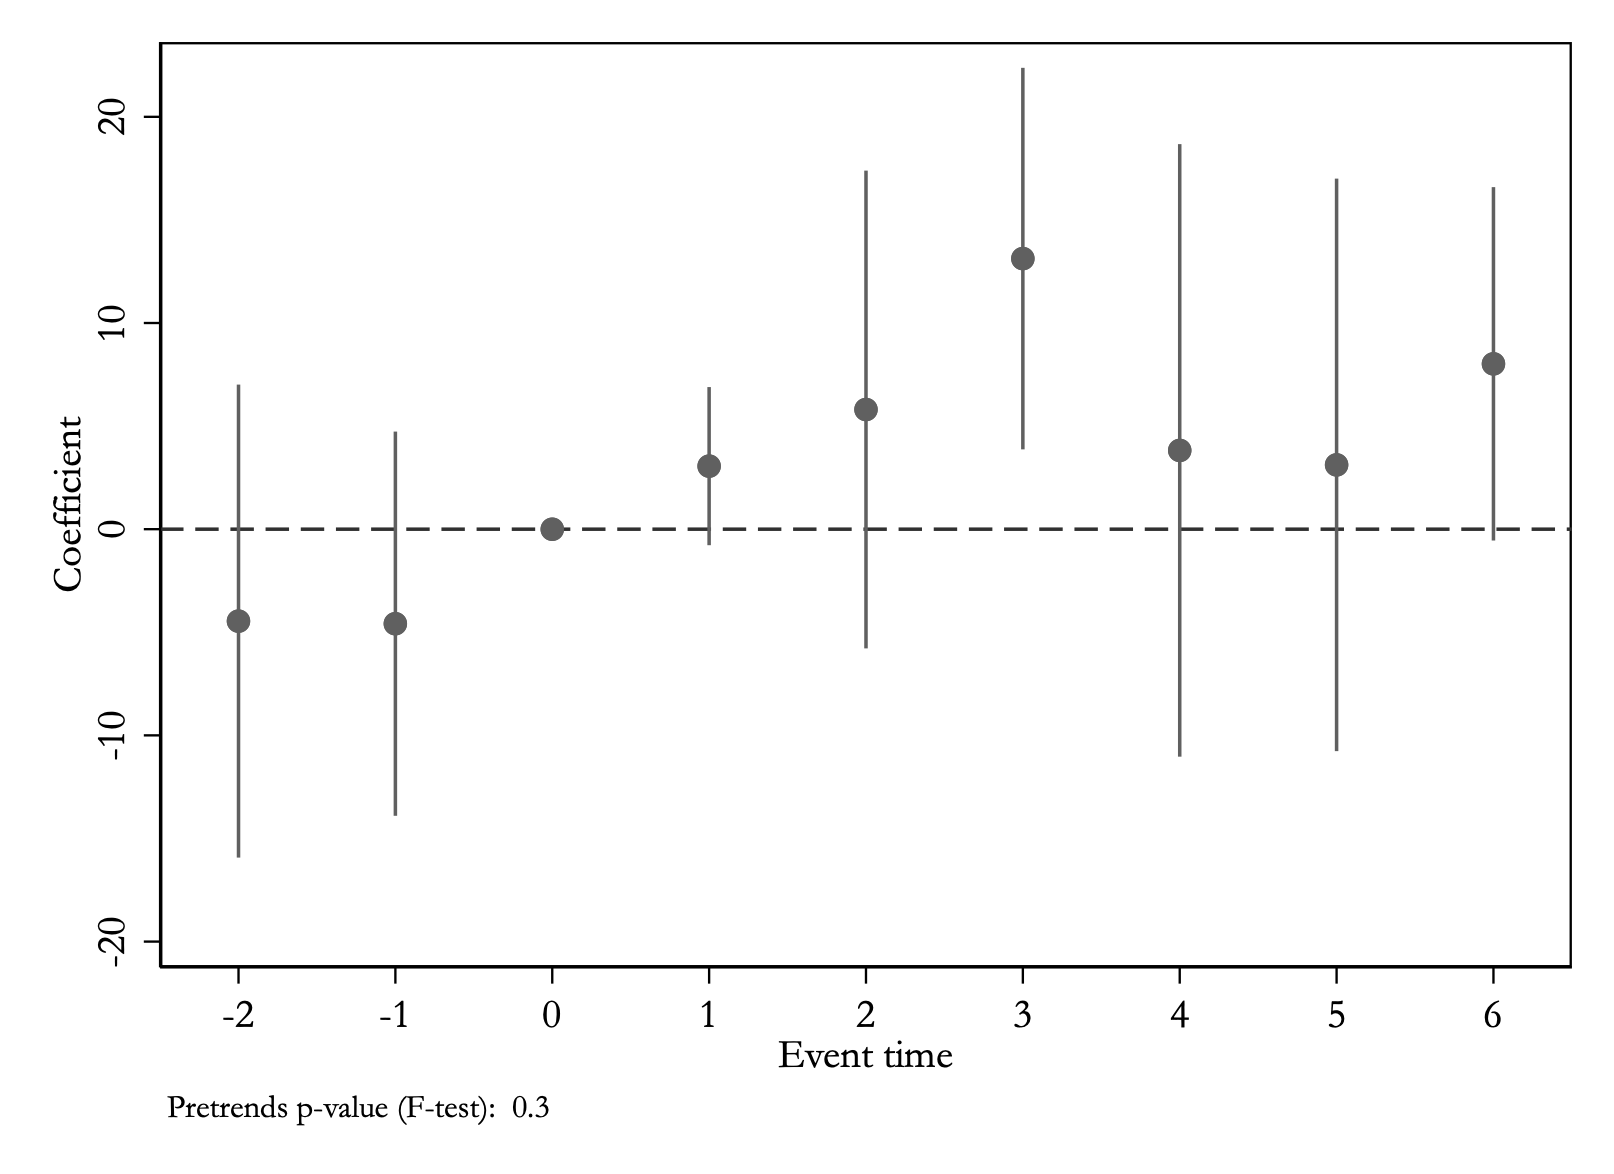
\includegraphics[width=0.7\textwidth]{eventstudy/high_drug_use/high_drug_eventstudy_1986.png}
    \label{fig:ab_es_1986}
  \end{figure}

  \begin{figure}[H]
    \caption{Effect of Anti-Drug Abuse Act on Drug-related Arrest Rate of Adult Black Men, Comparing States with High and Low Black Adult Drug-Related Arrest Rates (without Fixed Effects)}
    \centering
    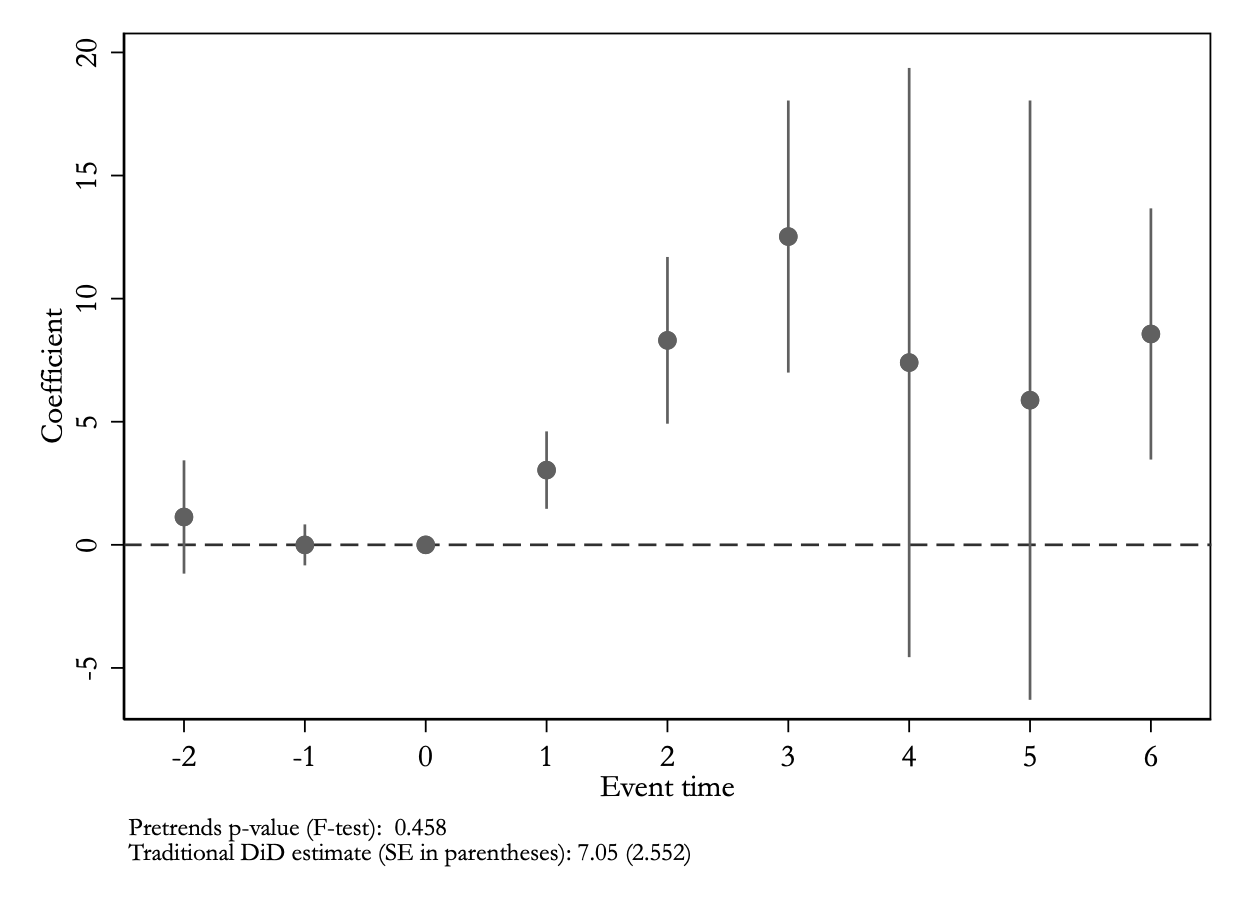
\includegraphics[width=0.7\textwidth]{eventstudy/high_drug_use/high_drug_eventstudy_nofe_1986.png}
    \label{fig:ab_es_1986_nofe}
  \end{figure}
  
  \begin{footnotesize}
    \noindent Note: This figure reports coefficients from the estimation of equation \ref{eq:state_level_es} evaluating the impact of the Anti-Drug Abuse Act of 1986 on arrest rates per 100,000 related to drug violations using CPS and UCR data from 1982-1992. Event time $0 \coloneqq 1986$. The coefficients represent the change in outcomes for high-drug arrest states relative to non-high-drug arrest states, where high black adult drug arrest states are defined to be those above the 75th percentile in 1984. The sample is defined as black males aged 18-24 in 1986 who were not incarcerated at the time of the survey. Control variables include population and unemployment rates at the state-year level. Right tail arrest rate outliers were winsorized at the 95\% level.
  \end{footnotesize}
  
  \clearpage

  \begin{figure}[h]
    \caption{Effect of Anti-Drug Abuse Act on Drug-related Arrest Rate of Black Men, Comparing States with High and Low Black Juvenile Drug-Related Arrest Rate}
    \centering
    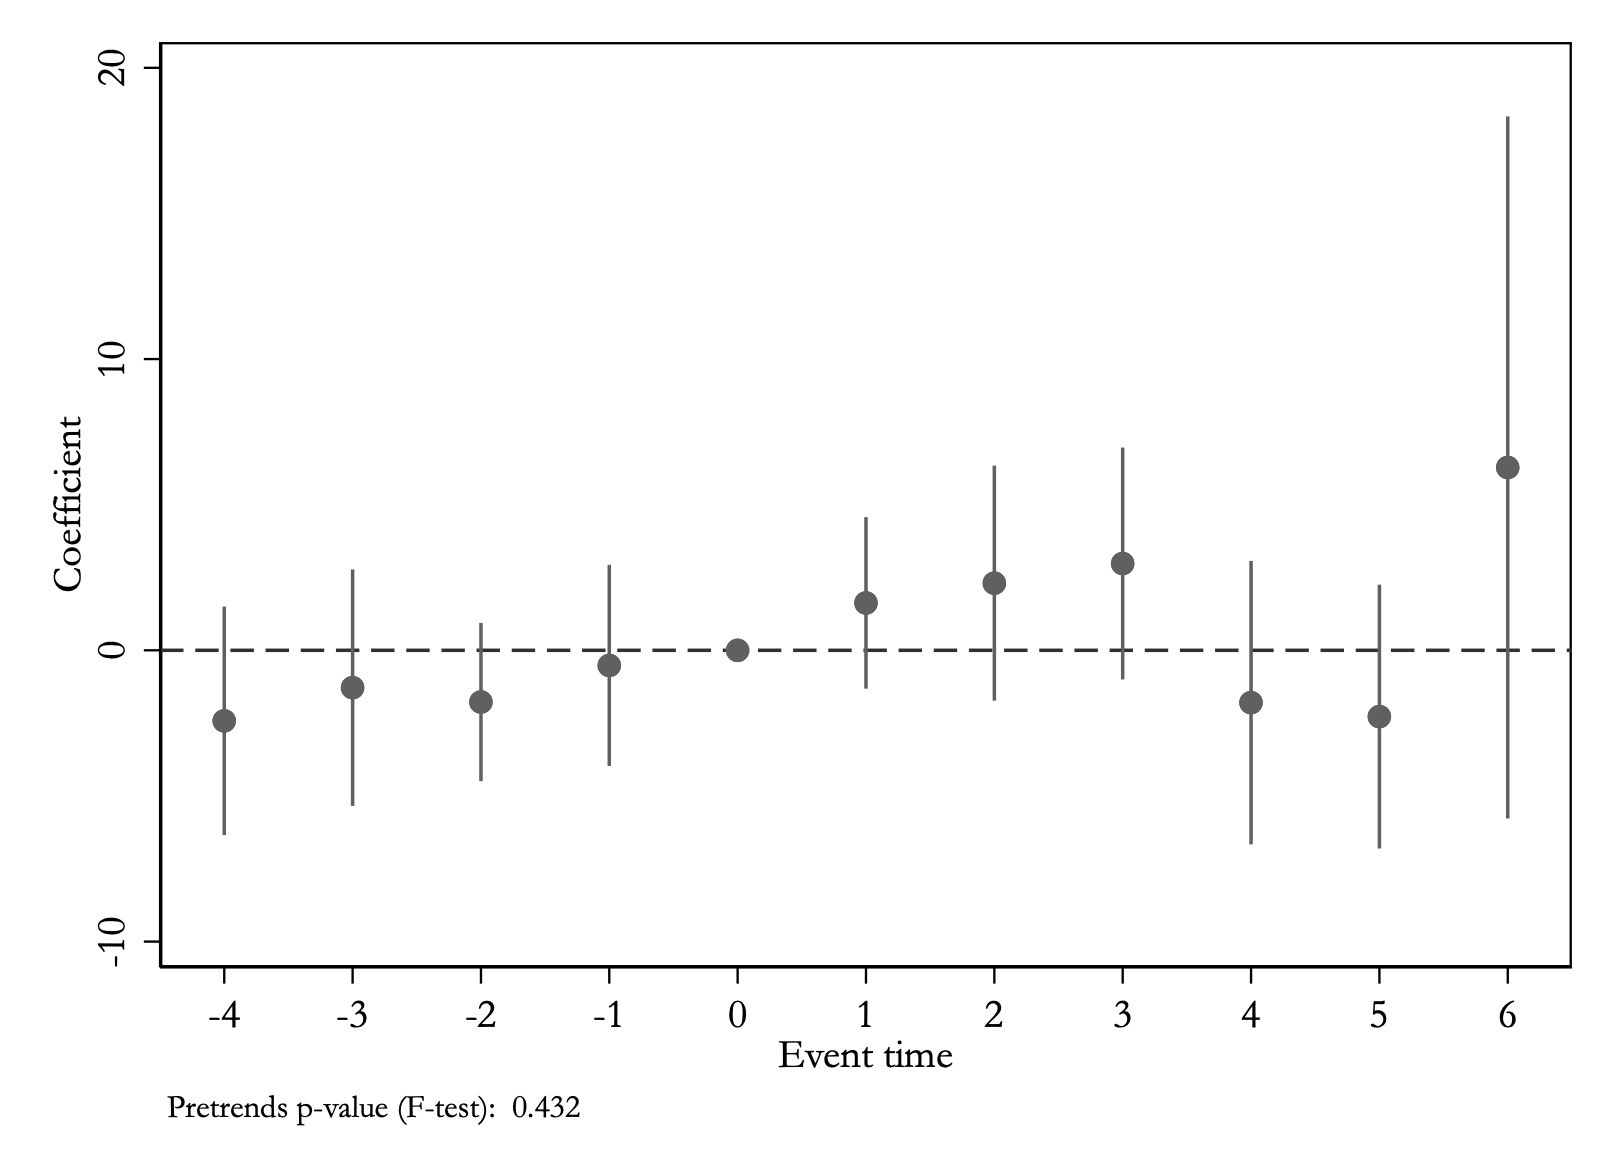
\includegraphics[width=1\textwidth]{eventstudy/high_drug_use/high_drug_eventstudy_1986_jb.png}
    \label{fig:jb_es_1986}
  \end{figure}

  \begin{footnotesize}
    \noindent Note: This figure reports coefficients from the estimation of equation 1 evaluating the impact of the Anti-Drug Abuse Act of 1986 on arrest rates per 100,000 related to drug violations using CPS and UCR data from 1982-1992. Event time $0 \coloneqq 1986$. The coefficients represent the change in outcomes for high black juvenile drug arrest states relative to non-high-drug arrest states, where high-drug arrest states are defined to be those above the 75th percentile in 1984. The sample is defined as black males aged 18-24 in 1986 who were not incarcerated at the time of the survey. Control variables include population and unemployment rates at the state-year level. 
  \end{footnotesize}

  \clearpage

  \begin{figure}[h]
    \centering
    \caption{Additional Pre-trend Testing for Coefficients from Figure 7}%
    \subfloat[\centering Linear pre-trend]{{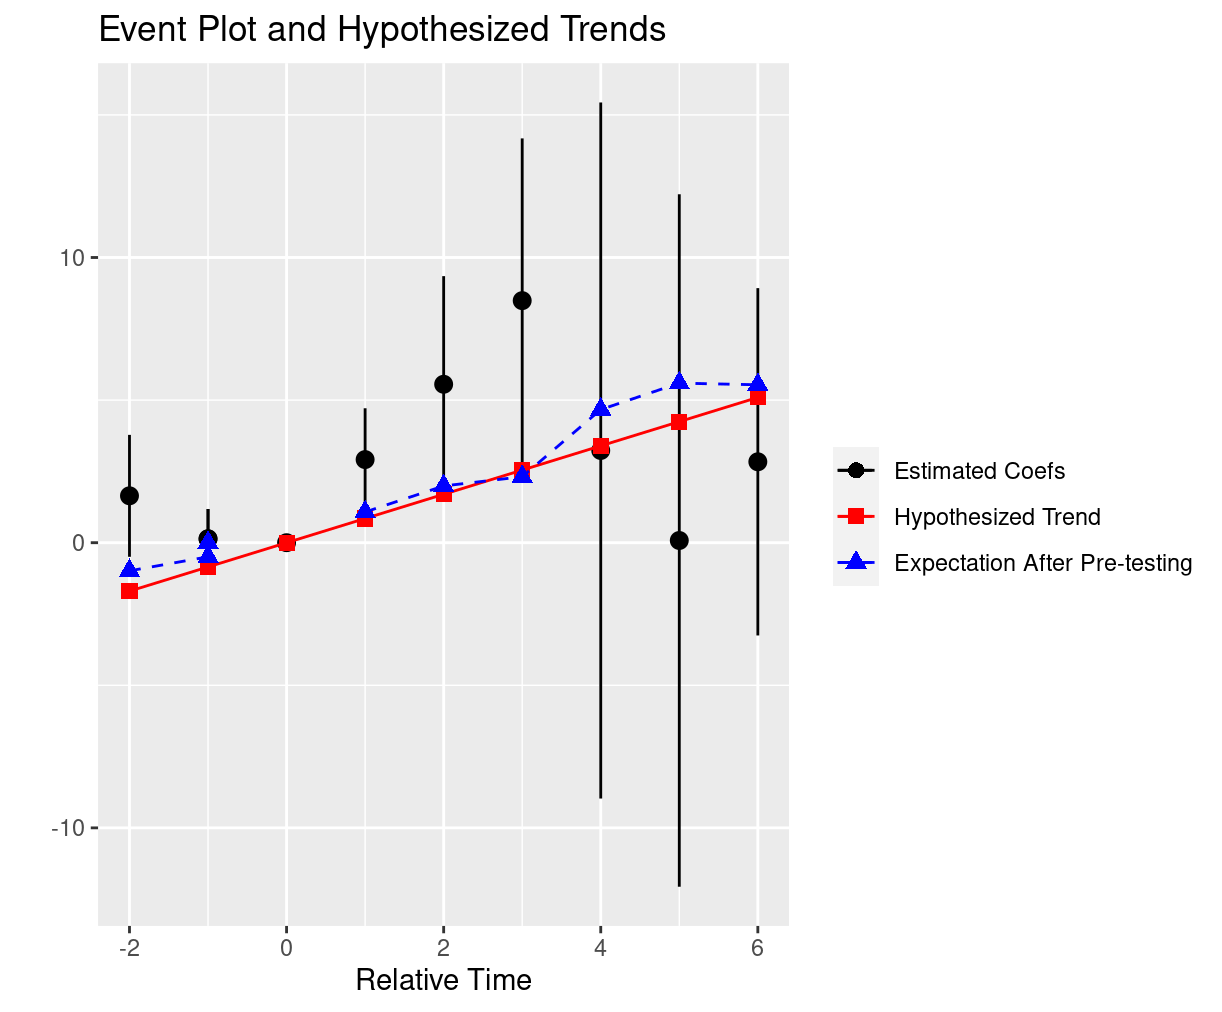
\includegraphics[width=7cm]{pretrends/power/firststage_linear_ab1986.png} }}%
    \qquad
    \subfloat[\centering Quadratic pre-trend]{{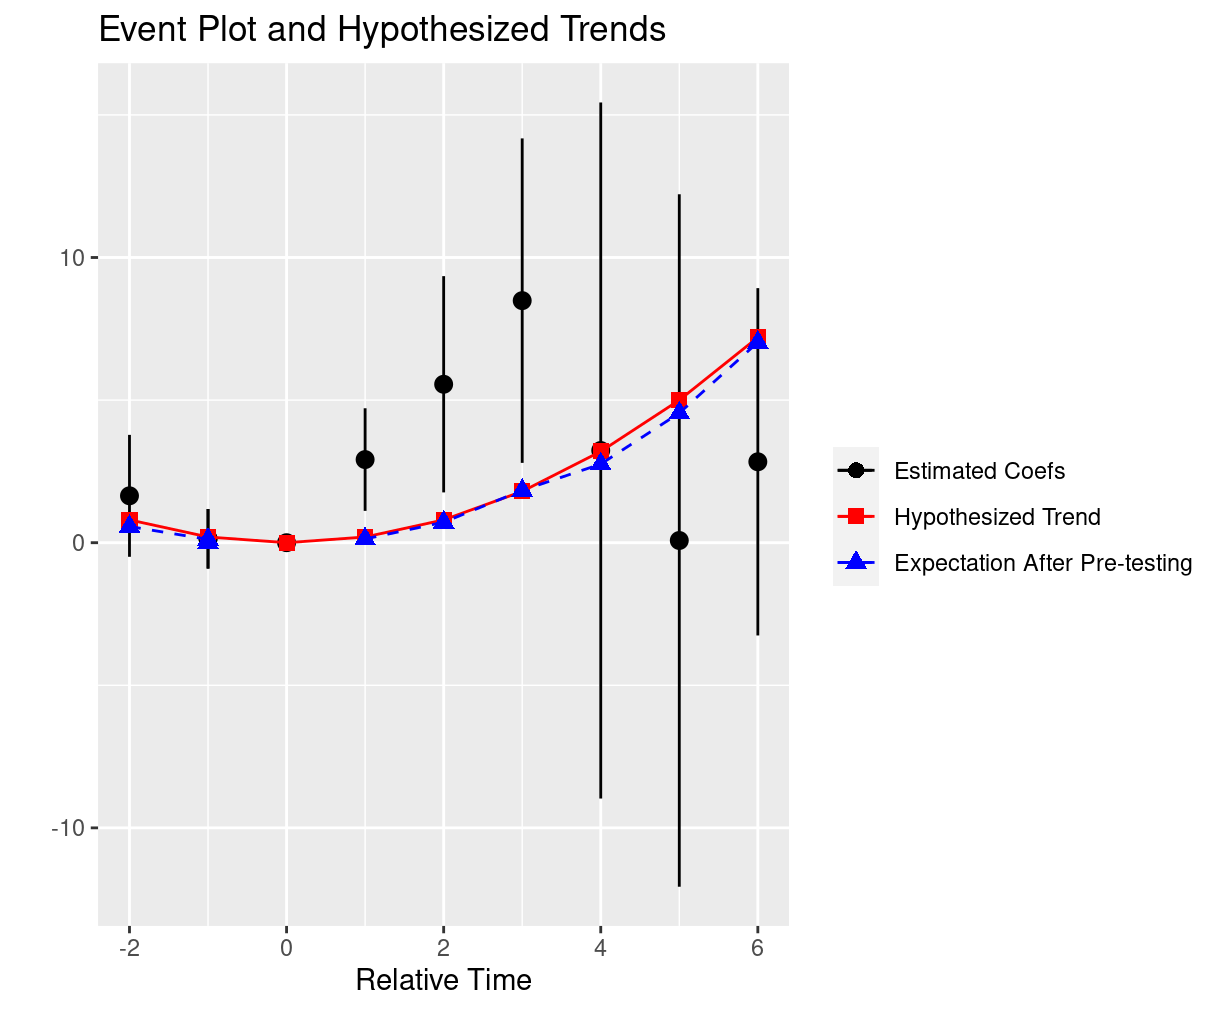
\includegraphics[width=7cm]{pretrends/power/firststage_quad_ab1986.png} }}%
    \label{fig:pre-trends_roth}%
  \end{figure}

  \begin{footnotesize}
    \noindent Note: These two figures were constructed using an R package written by Roth (2022). The figures and pre-trend statistics were calculated using the estimated coefficients from Figure 7 and their corresponding covariance matrixes. The slope in Figure A was constructed such that the power would be about 0.5, while the quadratic trend in Figure B was chosen visually. The blue expectation after pretesting coefficients represents the expected value of the coefficients conditional on passing the pre-test under the hypothesized trend.

    Figure A statistics: 1) power = 0.499, 2) Bayes Factor = 0.549, 3) likelihood ratio = 0.033.

    Figure B statistics: 1) power = 0.155, 2) Bayes Factor = 0.928, 3) likelihood ratio = 2.323.
  \end{footnotesize}

  \clearpage
  
  \begin{figure}[h]
    \centering
    \caption{Effect of Fair Sentencing Act on Drug-related Arrest Rate of Adult Black Men, Comparing High and Low-Intensity States}%
    \subfloat[\centering Using adults arrests]{{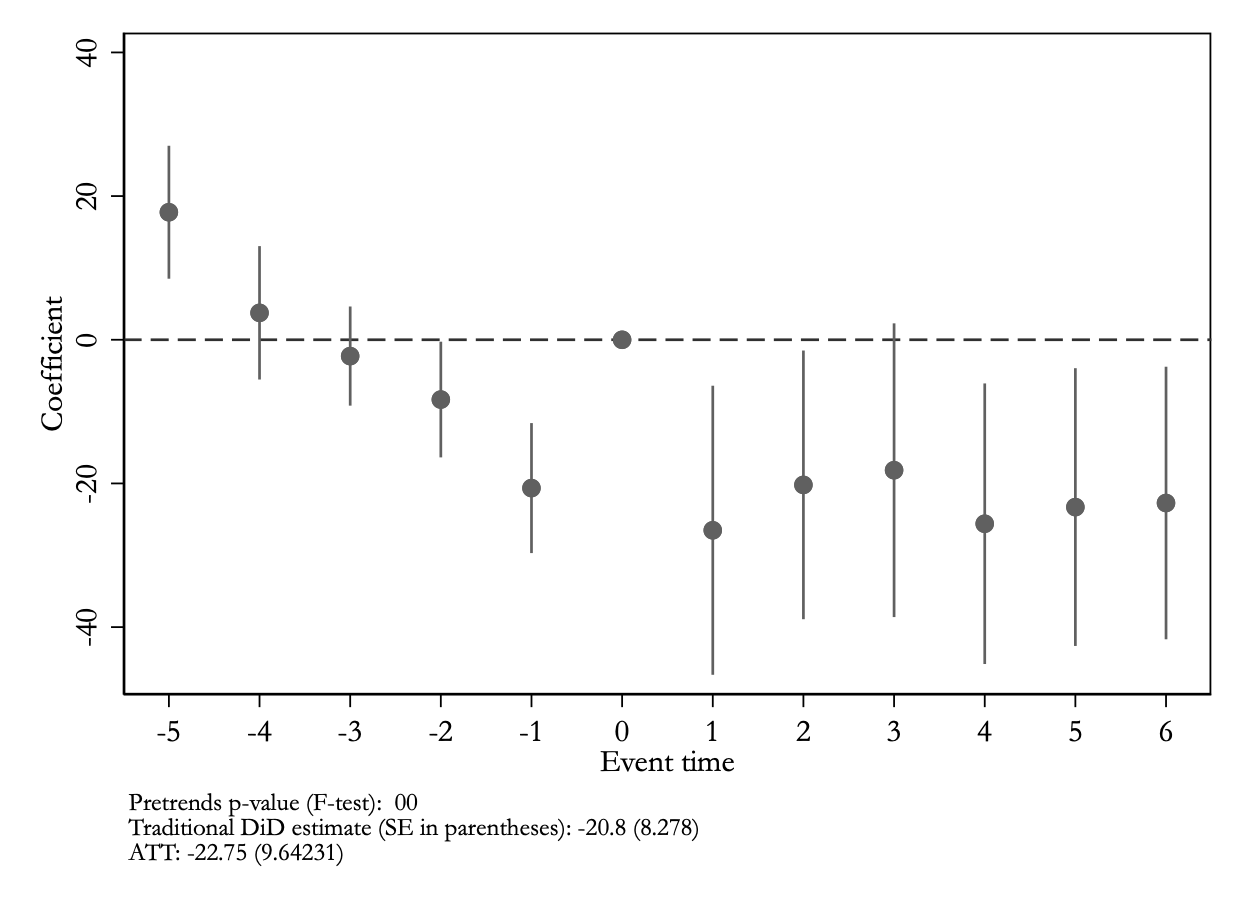
\includegraphics[width=7cm]{eventstudy/high_drug_use/high_drug_eventstudy_2010_ab.png} }}%
    \qquad
    \subfloat[\centering Using juvenile arrests]{{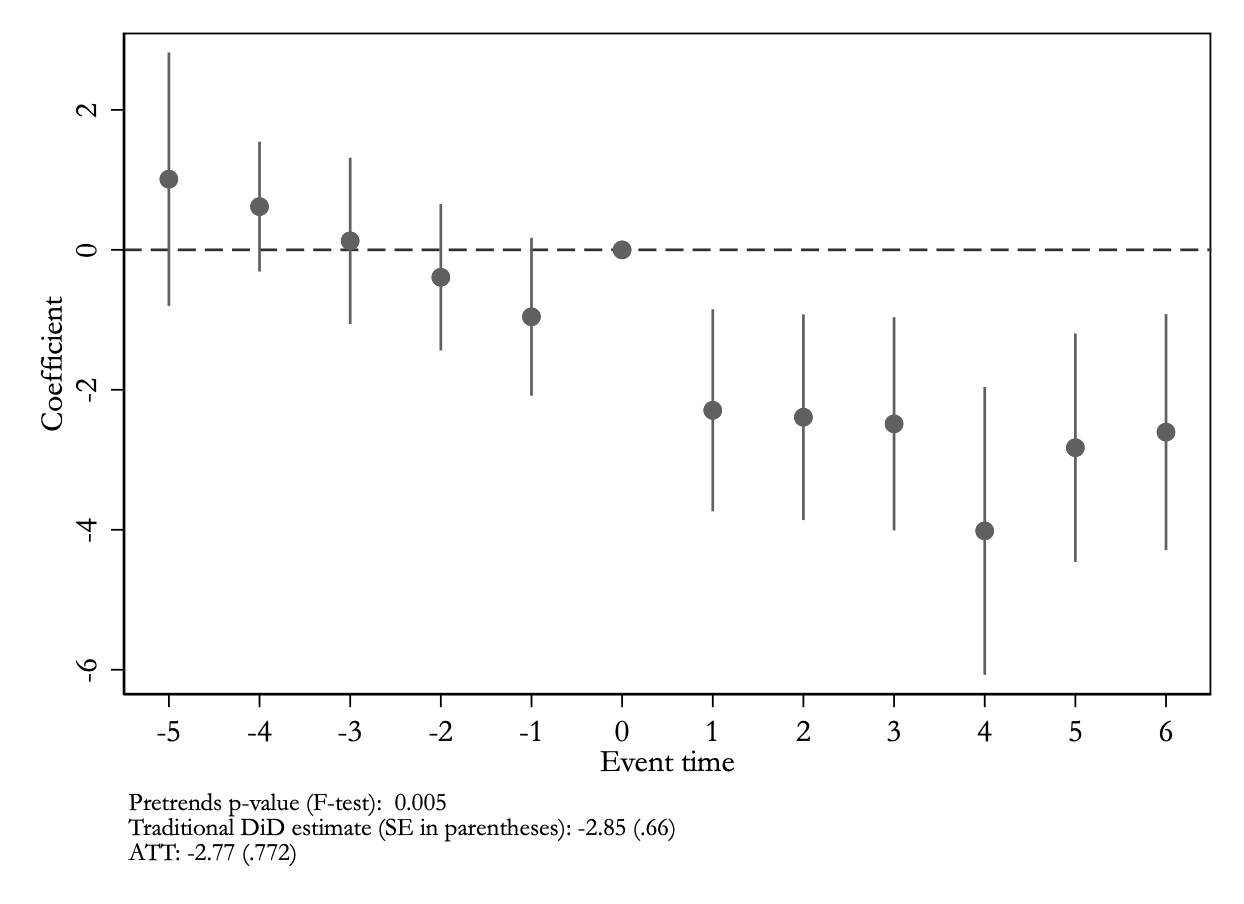
\includegraphics[width=7cm]{eventstudy/high_drug_use/high_drug_eventstudy_2010_jb.png} }}%
    \label{fig:fs_es_2010}%
  \end{figure}


  \begin{footnotesize}
    \noindent Note: These figures report coefficients from the estimation of equation 1 evaluating the impact of the Fair Sentencing Act of 2010 on arrest rates per 100,000 related to drug violations using CPS-UCR merged data from 2005-2015. Figure A defines high-intensity states using Black adult arrests, while Figure B defines high-intensity states using Black juvenile arrests. Event time $0 \coloneqq 2010$. The coefficients represent the change in outcomes for high black adult drug arrest states relative to non-high-drug arrest states, where high-drug arrest states are defined to be those above the 75th percentile in 2008. The sample is defined as black males aged 18-24 in 2010 who were not incarcerated at the time of the survey. Control variables include population and unemployment rates at the state-year level. 
  \end{footnotesize}

\clearpage 

\begin{figure}[h]
  \centering
  \caption{Effect of Anti-Drug Abuse Act on the College Enrollment Rate of Adult Black Men, Comparing High and Low-Intensity States}%
  \subfloat[\centering Using adults arrests]{{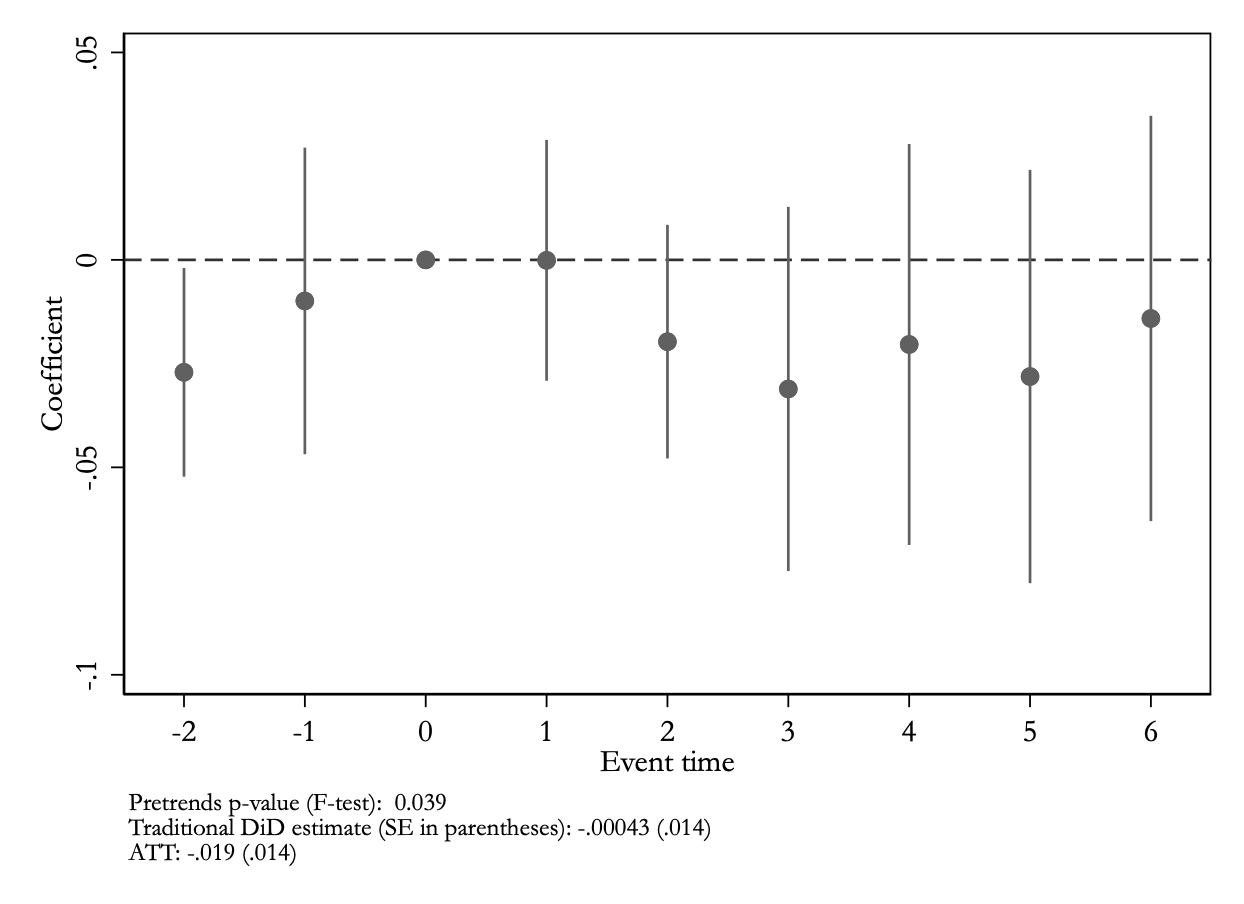
\includegraphics[width=7cm]{eventstudy/high_drug_use/reducedform_ab1986.png} }}%
  \qquad
  \subfloat[\centering Using juvenile arrests]{{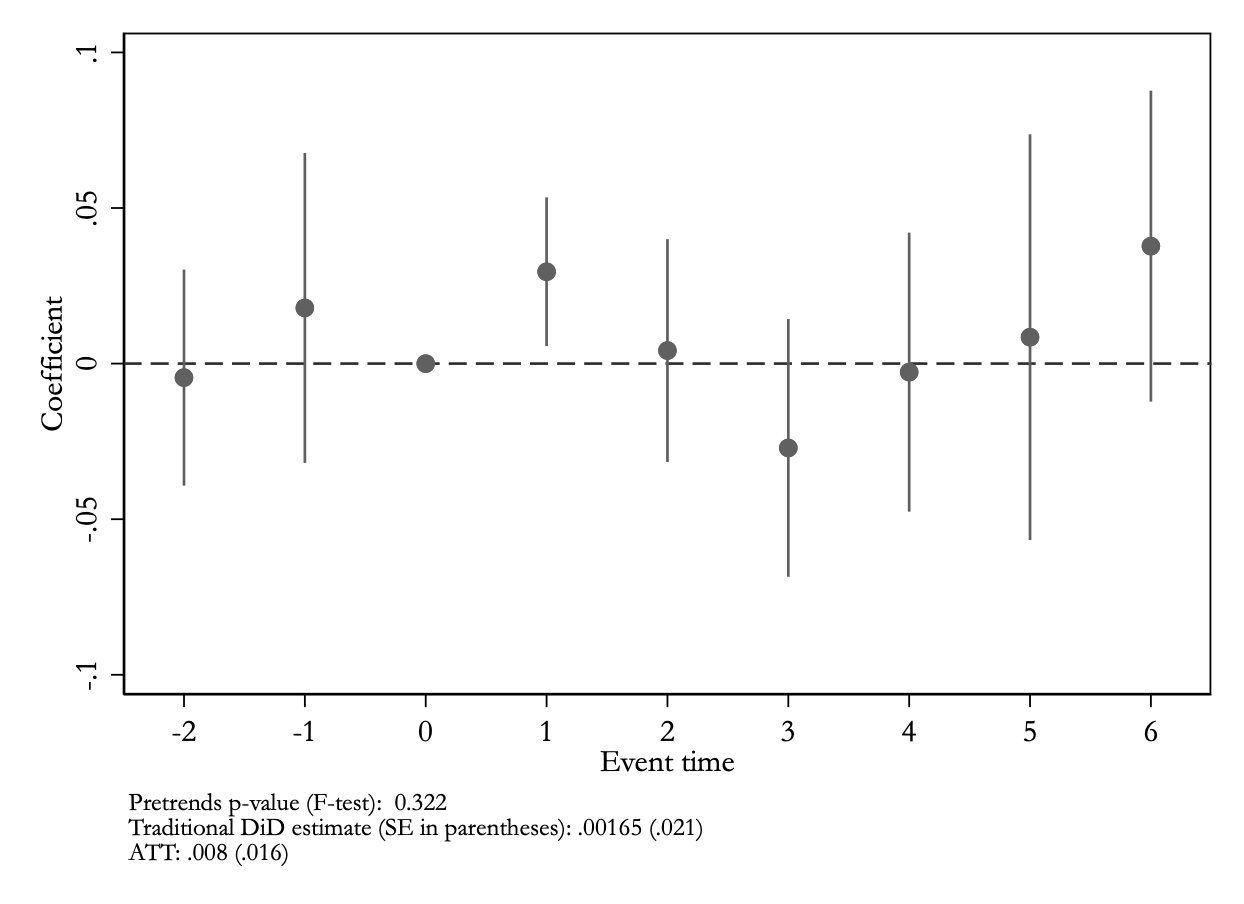
\includegraphics[width=7cm]{eventstudy/high_drug_use/reducedform_jb1986.png} }}%
  \label{fig:rs_es_1986}%
\end{figure}

\begin{footnotesize}
  \noindent Note: These figures report coefficients from the estimation of equation 1 evaluating the impact of the Anti-Drug Abuse Act of 1986 on college enrollment rates using CPS-UCR merged data from 1984-1992. Figure A defines high-intensity states using Black adult arrests, while Figure B defines high-intensity states using Black juvenile arrests. Event time $0 \coloneqq 1986$. The coefficients represent the change in outcomes for high black adult drug arrest states relative to non-high-drug arrest states, where high-drug arrest states are defined to be those above the 75th percentile in 1984. The sample is defined as black males aged 18-24 in 1986 who were not incarcerated at the time of the survey. Control variables include population and unemployment rates at the state-year level. 
\end{footnotesize}

\clearpage

\begin{figure}[h]
  \centering
  \caption{Effect of Fair Sentencing Act on the College Enrollment Rate of Adult Black Men, Comparing High and Low-Intensity States}%
  \subfloat[\centering Using adults arrests]{{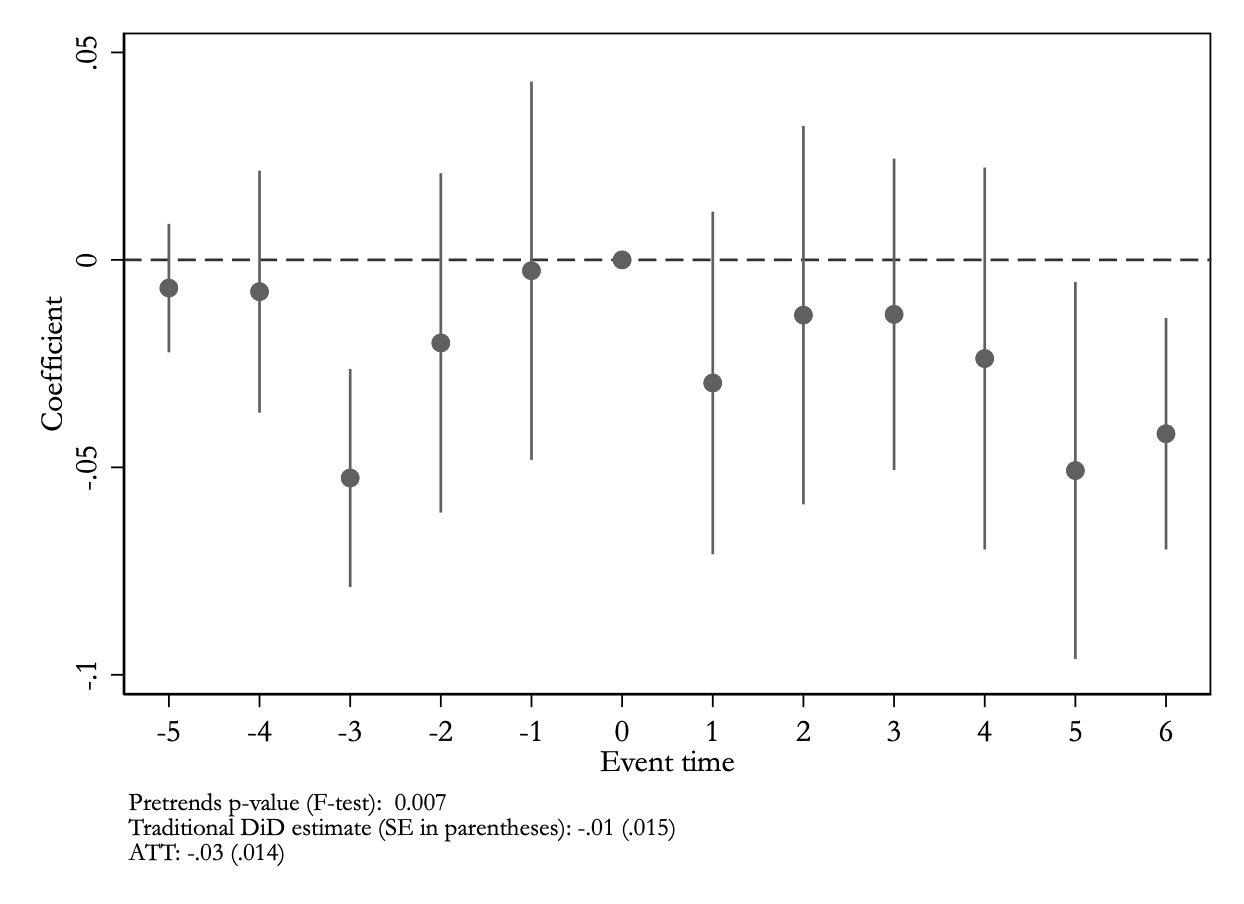
\includegraphics[width=7cm]{eventstudy/high_drug_use/reducedform_ab2010.png} }}%
  \qquad
  \subfloat[\centering Using juvenile arrests]{{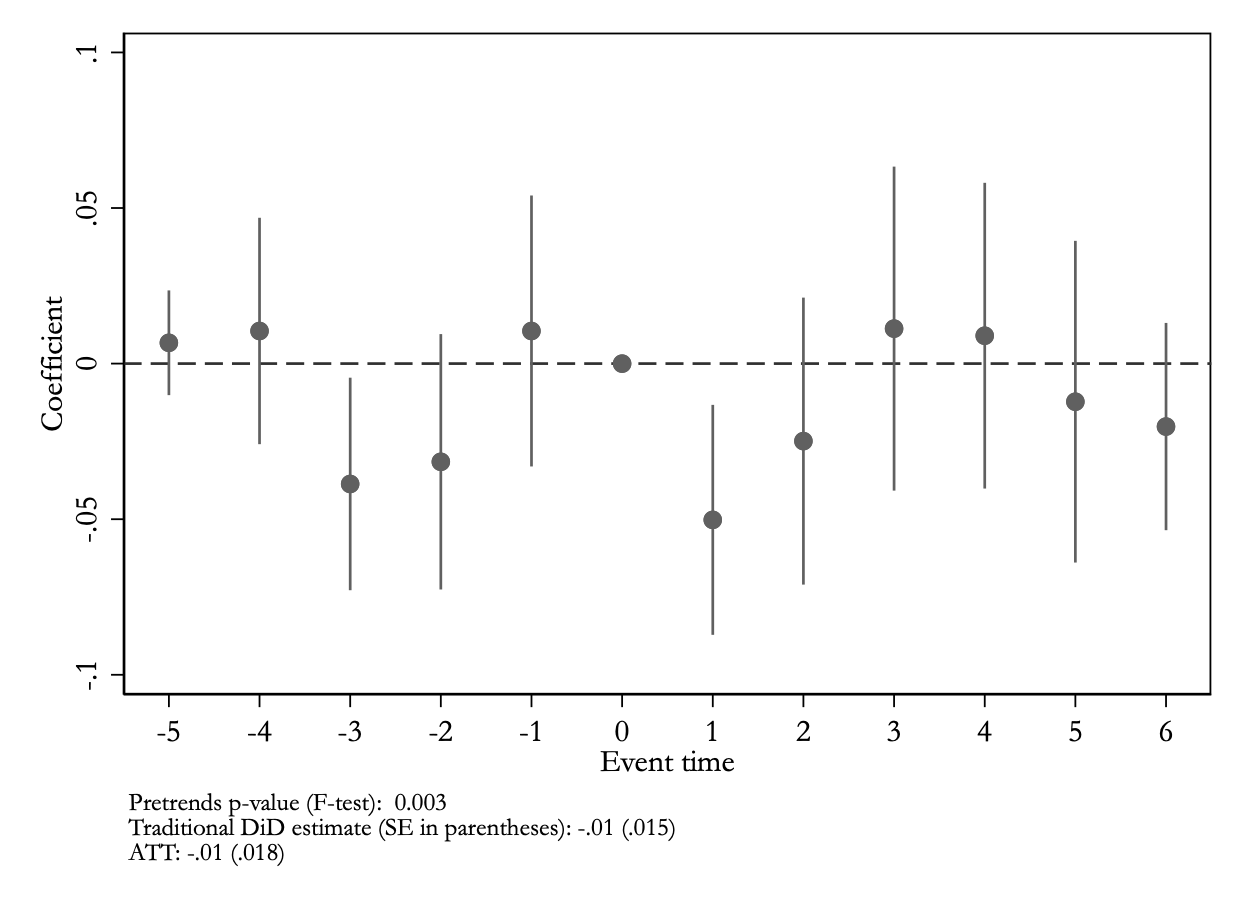
\includegraphics[width=7cm]{eventstudy/high_drug_use/reducedform_jb2010.png} }}%
  \label{fig:rf_jb_es_2010}%
\end{figure}

\begin{footnotesize}
  \noindent Note: These figures report coefficients from the estimation of equation 1 evaluating the impact of the Fair Sentencing Act of 2010 on college enrollment rates using CPS-UCR merged data from 2005-2015. Figure A defines high-intensity states using Black adult arrests, while Figure B defines high-intensity states using Black juvenile arrests. Event time $0 \coloneqq 2010$. The coefficients represent the change in outcomes for high black adult drug arrest states relative to non-high-drug arrest states, where high-drug arrest states are defined to be those above the 75th percentile in 2008. The sample is defined as black males aged 18-24 in 2010 who were not incarcerated at the time of the survey. Control variables include population and unemployment rates at the state-year level. 
\end{footnotesize}

\clearpage


%%%%%%%%%%%%%%%%%%%%%%%%TABLES%%%%%%%%%%%%%%%%%%%%%%%%%%%
\clearpage


\import{../../output/tables/summ_stats/}{cps_ucr_summ_stats.tex}

\begin{footnotesize}
  \noindent Note: Sample means with education supplement weights are calculated from the CPS-UCR merged dataset from 1984 to 1992 and 2000 to 2016. The sample in columns 1 and 2 is defined as persons aged 18-24 in 1986, and the sample in columns 3 and 4 is defined as persons aged 18-24 in 2010, both of whom were not incarcerated at the time of the survey.
\end{footnotesize}

\clearpage

\import{../../output/tables/ddiv}{ddiv_show2.tex}
\begin{footnotesize}
  \noindent Note: The CPS-UCR merged dataset is used for this table.  Mean estimates are weighted using CPS October supplement weights. No controls or fixed effects were used, and significance stars are omitted. Robust standard errors are clustered at the state level. The sample is defined as males aged 18-24 in 1986 who were not incarcerated at the time of the survey. 
\end{footnotesize}

\clearpage

\import{../../output/tables/ddiv}{iv.tex}
\begin{footnotesize}
  \noindent Note: The CPS-UCR merged dataset is used for this table. Estimates are weighted using CPS October supplement weights. The controls used at the individual level include age, age-squared, Latino ethnicity, and binned family income. The controls used at the state level include unemployment and population.
  Robust standard errors are clustered at the state level. The sample is defined as males aged 18-24 in 1986 who were not incarcerated at the time of the survey. 
\end{footnotesize}

\clearpage

%DiD High/low intensity 

\import{../../output/tables/}{DiD_1986_high_low.tex}
\begin{footnotesize}
  \noindent Note: Estimates are weighted using CPS October supplement weights. Robust standard errors are clustered at the state level. The controls used include age, age-squared, Latino ethnicity, yearly state average unemployment rates, and (binned) family income. The sample is defined as males aged 18-24 in 1986 who were not incarcerated at the time of the survey.
\end{footnotesize}

\import{../../output/tables/}{DiD_1986_high_low_cont.tex}
\begin{footnotesize}
  \noindent Note: Estimates are weighted using CPS October supplement weights. Robust standard errors are clustered at the state level. Controls: age, age-squared, Latino ethnicity, yearly state average unemployment rates, and (binned) family income. The sample is defined as males aged 18-24 in 1986 who were not incarcerated at the time of the survey.
\end{footnotesize}
\clearpage

\import{../../output/tables/}{DiD_1986_high_low_jb.tex}
\begin{footnotesize}
  \noindent Note: Estimates are weighted using CPS October supplement weights. Robust standard errors are clustered at the state level. The controls used include age, age-squared, Latino ethnicity, yearly state average unemployment rates, and (binned) family income. The sample is defined as males aged 18-24 in 1986 who were not incarcerated at the time of the survey.
\end{footnotesize}

\import{../../output/tables/}{DiD_1986_high_low_jb_cont.tex}
\clearpage

\import{../../output/tables/}{DiD_1986_high_low_jb_cont_control_experiment_female.tex}


\import{../../output/tables/}{DiD_1986_high_low_jb_cont_control_experiment_old.tex}

\clearpage

\import{../../output/tables/}{DiD_2010_high_low.tex}
\begin{footnotesize}
  \noindent Note: Treated observations are defined as those living in states with a high-drug arrest rate for black adults, where high black adult drug arrest states are defined to be those above the 75th percentile in 2008. Estimates are weighted using CPS October supplement weights. Robust standard errors are clustered at the state level. Controls: age, age-squared, Latino ethnicity, yearly state average unemployment rates, and (binned) family income. The sample is defined as males aged 18-24 in 1986 who were not incarcerated at the time of the survey.
\end{footnotesize}

\import{../../output/tables/}{DiD_2010_high_low_cont.tex}
\begin{footnotesize}
  \noindent Note: Treatment is continuous. Estimates are weighted using CPS October supplement weights. Robust standard errors are clustered at the state level. Controls: age, age-squared, Latino ethnicity, yearly state average unemployment rates, and (binned) family income. The sample is defined as males aged 18-24 in 2010 who were not incarcerated at the time of the survey.
\end{footnotesize}
\clearpage

% Britton Table 2
\import{../../output/tables/}{britton_table2_DiD.tex}
\begin{footnotesize}
  \noindent Note: Estimates are weighted using CPS October supplement weights. Robust standard errors are clustered at the state level. The controls used include age, age-squared, Latino ethnicity, and binned family income. The sample is defined as Black and White males aged 18-24 in 1986 who were not incarcerated at the time of the survey.
  This table is partially replicated from \cite{britton2022}.
\end{footnotesize}

\import{../../output/tables/}{britton_table3_DiD.tex}
\begin{footnotesize}
  \noindent Note: Estimates are weighted using CPS October supplement weights. Robust standard errors are clustered at the state level. The controls used include age, age-squared, Latino ethnicity, and binned family income. The sample is defined as Black males and Black females aged 18-24 in 1986 who were not incarcerated at the time of the survey. This table is partially replicated from \cite{britton2022}.
\end{footnotesize}

\clearpage

\import{../../output/tables/}{britton_table2_DiD_control_experiment.tex}
\begin{footnotesize}
  \noindent Note: Estimates are weighted using CPS October supplement weights. Robust standard errors are clustered at the state level. The controls used include age, age-squared, Latino ethnicity, and binned family income. The sample is defined as Black and White males aged 30-50 in 1986 who were not incarcerated at the time of the survey.
  This table is a control experiment for table 2 in \cite{britton2022}.
\end{footnotesize}

\import{../../output/tables/}{britton_table3_DiD_control_experiment.tex}
\begin{footnotesize}
  \noindent Note: Estimates are weighted using CPS October supplement weights. Robust standard errors are clustered at the state level. The controls used include age, age-squared, Latino ethnicity, and binned family income. The sample is defined as Black males and Black females aged 30-50 in 1986 who were not incarcerated at the time of the survey.
  This table is a control experiment for table 3 in \cite{britton2022}.
\end{footnotesize}
\clearpage

\import{../../output/tables/}{fair_sentencing_DiD_t1.tex}
\begin{footnotesize}
  \noindent Note: Estimates are weighted using CPS October supplement weights. Robust standard errors are clustered at the state level. The controls used include age, age-squared, Latino ethnicity, and binned family income. The sample is defined as Black and White males aged 18-24 in 2010 who were not incarcerated at the time of the survey.
\end{footnotesize}

\import{../../output/tables/}{fair_sentencing_DiD_t2.tex}
\begin{footnotesize}
  \noindent Note: Estimates are weighted using CPS October supplement weights. Robust standard errors are clustered at the state level. The controls used include age, age-squared, Latino ethnicity, and binned family income. The sample is defined as Black males and females aged 18-24 in 2010 who were not incarcerated at the time of the survey.
\end{footnotesize}

\import{../../output/tables/}{fair_sentencing_DiD_t1_control_experiment.tex}
\begin{footnotesize}
  \noindent Note: Estimates are weighted using CPS October supplement weights. Robust standard errors are clustered at the state level. The controls used include age, age-squared, Latino ethnicity, and binned family income. The sample is defined as Black and White males aged 30-50 in 2010 who were not incarcerated at the time of the survey.
\end{footnotesize}

\import{../../output/tables/}{fair_sentencing_DiD_t2_control_experiment.tex}
\begin{footnotesize}
  \noindent Note: Estimates are weighted using CPS October supplement weights. Robust standard errors are clustered at the state level. The controls used include age, age-squared, Latino ethnicity, and binned family income. The sample is defined as Black males and females aged 30-50 in 2010 who were not incarcerated at the time of the survey.
\end{footnotesize}
\clearpage

\import{../../output/tables/ddd}{ddd_1986_ab.tex}
\begin{footnotesize}
  \noindent Note: CPS data from 1984-1992.
  The sample is defined as males aged 18-24 in 1986 who were not incarcerated at the time of the survey.
\end{footnotesize}

\clearpage

\import{../../output/tables/ddd}{ddd_1986_jb.tex}

\clearpage

\import{../../output/tables/ddd}{ddd_2010_ab.tex}

\clearpage

\import{../../output/tables/ddd}{ddd_2010_jb.tex}
\clearpage 




%%%%%%%%%%%%%%%%%%%%%%%%APPENDIX%%%%%%%%%%%%%%%%%%%%%%%%%%%
\clearpage

\begin{appendices}
  \section{Additional Results}
  The contents...
  \section{section 2}
\end{appendices}





\end{document}
